\documentclass[conference,onecolumn]{IEEEtran}
\IEEEoverridecommandlockouts
\usepackage{amsmath,amssymb,amsfonts}
\usepackage{algorithmic}
\usepackage{algorithm}
\usepackage[pdftex]{graphicx}
\usepackage{textcomp}
\usepackage{xcolor}
% Generated by tools/analysis/model_palette.py. Do not edit manually.
\definecolor{modelM0}{HTML}{D55E00}
\definecolor{modelM1}{HTML}{8C9AA9}
\definecolor{modelM2}{HTML}{A7B6C2}
\definecolor{modelM3}{HTML}{6B8DB5}
\definecolor{modelM4}{HTML}{E69F00}
\definecolor{modelM5}{HTML}{F0C04A}
\definecolor{modelM6}{HTML}{7CB342}
\definecolor{modelM7}{HTML}{56B4E9}
\definecolor{modelM8}{HTML}{CC79A7}
\definecolor{modelM9}{HTML}{0072B2}
\definecolor{modelM9RF2}{HTML}{009E73}
\definecolor{supplementalNeutral}{HTML}{6B7C93}
\newcommand{\modelid}[2]{%
  \raisebox{0.15ex}{\textcolor{#1}{\rule{0.85ex}{0.85ex}}}\nobreakspace\textbf{#2}%
}

\usepackage{flushend}
\usepackage{hyperref}
\hypersetup{hidelinks}
\usepackage{pdflscape}
\usepackage{tabularray}
\usepackage{cite}
\usepackage{booktabs}
\usepackage{url}
\usepackage{multirow}
\usepackage{array}
\usepackage{placeins}
\usepackage{float}

\title{Flow is All You Need for WiFi: Rectifying 3D Human Poses without Complex Architectures}

\author{
Nguyen Vinh Nghi,  Le Ngoc Anh Thu,  Nguyen Ngo Nhat Nam, and Tran Ngoc Hoang\\
FPT University, Ho Chi Minh Campus, Vietnam\\
\{CE182108, CE180615, CE181939\}@fpt.edu.vn, and hoang2531992@gmail.com}

\begin{document}
\maketitle

\begin{abstract}
WiFi-based human pose estimation offers an occlusion-resilient alternative to camera-based sensing, but estimating multi-person 3D skeletons from channel state information remains difficult because WiFi signals are noisy, low-dimensional, and strongly affected by multipath propagation. This paper presents a compact draft-to-refine architecture that combines spectrally conditioned temporal residual tokens, flattened Mamba-2 sequence modeling, a lightweight query-pose head, and conditional flow correction. A controlled M0--M9 ladder separates representation, encoder, pose-head, and refinement effects. On a public fixed-layout CSI--RGB-D benchmark \cite{yan2024personwifi3d}, Mamba-2 Flow (two steps) achieves 165.487 mm MPJPE at 209.9 FPS with 3.618M parameters and 25.29 MB peak allocated memory. Relative to the Transformer-PETR control, this operating point reduces MPJPE by 7.053 mm (4.09\%), increases throughput from 118.7 FPS, and reduces model size and allocated memory from 13.130M parameters and 155.60 MB. These results support a scoped architectural claim: after compact CSI encoding and draft prediction, a small two-step flow stage provides the correction needed to reach the lowest error in the evaluated ladder without a complex pose decoder.
\end{abstract}

\begin{IEEEkeywords}
WiFi sensing, CSI, 3D human pose estimation, Mamba2, flow matching, spectral tokenization.
\end{IEEEkeywords}

\section{Introduction}
WiFi channel state information (CSI) provides a non-visual sensing signal that can be used for human perception in indoor environments. Unlike camera-based pose estimation, WiFi sensing can operate under occlusion and low-light conditions, but the input is indirect: body motion perturbs multipath propagation rather than producing explicit visual evidence. This makes multi-person 3D pose estimation from WiFi substantially harder than pose estimation from images.

Our design hypothesis is that efficient WiFi pose estimation does not require a large pose-decoding stack when the model first produces a compact, query-conditioned draft and then corrects its coordinates with a small learned flow field. We test this hypothesis through an architecture ladder that separates spectral tokenization, Transformer and Mamba-family sequence encoders, PETR and lightweight query-pose heads, and draft-only versus flow-refined inference. The selected configuration combines spectral tokenization, a flattened Mamba-2 encoder, a lightweight query-pose head, and two Euler correction steps.

The initial proposal formulated representation, efficient sequence modeling, flow correction, and final operating-point selection as coupled hypotheses. The full study expands those hypotheses into controlled M0--M9 comparisons so that the contribution of each input, encoder, pose-head, and refinement choice can be inspected independently. M9\_RF2 is the measured final operating point of this expanded ablation rather than a configuration assumed in advance.

The study uses a public fixed-layout CSI--RGB-D benchmark and its published temporal split \cite{yan2024personwifi3d}. It therefore evaluates compact architecture choices under a shared three-receiver sensing and evaluation protocol; cross-person and cross-environment generalization are outside the scope of this ablation.

The contributions are:
\begin{itemize}
    \item a Spectrally Conditioned Temporal Residual Tokenizer (shortened to \emph{Spectral Tokenizer}) that uses a compact projected-feature spectral descriptor to condition a per-link temporal residual update;
    \item a compact flattened Mamba-2 and lightweight query-pose path that establishes the 247.7 FPS, 1.813M-parameter efficiency endpoint;
    \item a conditional two-step flow correction that reaches the lowest measured MPJPE, 165.487 mm, while retaining 209.9 FPS. To the best of our knowledge, this is the first WiFi-based multi-person 3D pose framework to use conditional flow matching as a learned draft-to-pose correction mechanism.
    \item a controlled M0--M9 study reporting scene-cardinality accuracy, matched and missed-person behavior, throughput, parameters, and peak allocated memory under one shared protocol.
\end{itemize}

\section{Related Work}
\subsection{Human Pose from Images}
\label{sec:related-camera}
Camera-based pose estimation supplies the structural precedents used by WiFi pose systems \cite{zheng2023posesurvey}. Bottom-up methods such as OpenPose regress keypoint heatmaps and part affinity fields before grouping joints into people \cite{cao2017openpose}; top-down methods detect each person before applying a single-person estimator, as in AlphaPose \cite{fang2017alphapose}. HRNet preserves high-resolution spatial features for keypoint localization \cite{sun2019hrnet}. DETR later formulated detection as direct set prediction with learned queries and bipartite matching \cite{carion2020detr}, and PETR adapted that formulation to multi-person pose regression \cite{shi2022petr}. Our decoder inherits the query-set abstraction, but its input is CSI rather than spatially localized image evidence.

\subsection{WiFi-based 2D Human Pose Estimation}
Early WiFi pose systems mapped channel measurements to image-like supervision. Person-in-WiFi predicts joint heatmaps and part affinity fields, then groups them into multiple 2D skeletons without using an RGB image at inference \cite{wang2019personwifi2d}. EASFN combines spatial--frequency feature extraction with evolving attention for WiFi-based multi-person 2D pose estimation \cite{chen2023easfn}. These methods establish that CSI can support joint association, but a 2D skeleton does not encode metric depth and therefore cannot directly represent a person in 3D space.

\subsection{WiFi-based Single-Person 3D Pose Estimation}
Single-person 3D studies have explored complementary signal representations and structural priors. WiPose learns person-independent 3D coordinate regression from CSI dynamics \cite{jiang2020wipose}; WiNect and GoPose use temporal information for free-form 3D tracking \cite{ren2021winect,ren2022gopose}. MetaFi++ targets device-free avatar pose estimation, whereas HPE-Li emphasizes lightweight inference \cite{zhou2023metafiplus,gian2024hpeli}. PowerSkel introduces an application-specific skeleton estimator for industrial environments, and GraphPose-Fi uses graph structure to model joint dependencies \cite{yin2024powerskel,chen2025graphwifi}. MM-Fi complements these methods with a multimodal benchmark that includes 3D pose labels for wireless sensing research \cite{yang2023mmfi}. Together, this literature covers coordinate regression, temporal tracking, efficient models, and skeletal topology, but it generally assumes one pose instance per input.

\subsection{WiFi-based Multi-Person 3D Pose Estimation}
WiFi-based multi-person 3D pose estimation remains a nascent area represented by a still-small set of studies. The CVPR 2024 query-based formulation established direct multi-person 3D set prediction from WiFi CSI through learned pose queries and Hungarian matching \cite{yan2024personwifi3d}. WiFi-Mamba subsequently introduced interleaved selective state-space modeling for efficient multi-person 3D WiFi pose estimation \cite{nguyen2026wifimamba}. Because their training schedules, checkpoints, and evaluators are not interchangeable, we do not make cross-paper numerical comparisons. We make no novelty claim about using Mamba or addressing multi-person 3D WiFi pose itself. The distinction examined here is the controlled combination of a flattened Mamba-2 encoder, compact query drafting, and flow-based coordinate correction across the M0--M9 ladder.

\subsection{Frequency-Aware CSI Representation and Feature Recalibration}
Frequency-aware processing has two distinct lineages relevant to CSI sensing. Signal-oriented systems construct physically interpretable representations: Widar3.0 derives body-coordinate velocity profiles for cross-domain gesture recognition, while SLNet jointly learns super-resolution spectrogram construction and downstream wireless features \cite{zhang2021widar3,yang2023slnet}. Within WiFi pose estimation, EASFN combines spatial--frequency feature extraction with evolving attention for multi-person 2D pose recovery \cite{chen2023easfn}. These methods motivate frequency-aware processing, but their velocity profiles, learned spectrograms, and image-like pose features are not the representation used here.

Fourier operations also appear in general sequence modeling. FNet replaces attention-based token mixing with Fourier transforms; FEDformer uses frequency-enhanced decomposition for long-horizon forecasting; and TimesNet identifies temporal periods in the frequency domain before organizing time series as two-dimensional variations \cite{lee2022fnet,zhou2022fedformer,wu2023timesnet}. A complementary lineage concerns learned feature recalibration: squeeze-and-excitation maps pooled descriptors through a small gating network, FcaNet extends channel descriptors with frequency components, and ReZero studies zero-initialized residual learning \cite{hu2018senet,qin2021fcanet,bachlechner2021rezero}. These are architectural precedents rather than direct WiFi-pose templates.

Our Spectral Tokenizer is therefore a task-specific composition of established operations, not a claim to have invented Fourier analysis, frequency attention, or zero-initialized residuals. It computes a one-sided magnitude descriptor from projected per-link CSI tokens, uses that descriptor to condition a temporal residual branch, and returns the update to the token sequence. Because the descriptor is computed after learned projection and is not calibrated to physical velocity, we do not interpret it as a Doppler spectrum or a spectrogram. Cross-paper numerical comparison would also be inappropriate because the cited methods differ in sensing task, signal processing, and evaluation protocol.

\subsection{Mamba and Mamba-2 for Pose and Wireless Sensing}
Mamba uses input-dependent selective state-space recurrence to model long sequences with linear scaling in sequence length \cite{gu2023mamba}. Mamba-2 derives an attention--state-space duality and an efficient structured state-space implementation \cite{dao2024mamba2}. Selective scans have since been adapted to visual representations by VMamba \cite{liu2024vmamba}, while PoseMamba applies state-space modeling to monocular 3D pose estimation \cite{huang2025posemamba}. SenseMamba studies selective state spaces for wireless sensing, and WiFi-Mamba specializes them for multi-person 3D WiFi pose \cite{huang2025sensemamba,nguyen2026wifimamba}. Our use of Mamba-2 is consequently not a standalone novelty claim: it is evaluated as the flattened sequence component of a compact draft-and-correct pipeline.

\subsection{Diffusion and Flow Matching for Pose Refinement}
Diffusion-based 3D pose methods treat pose recovery as iterative denoising. DiffPose generates pose hypotheses through a reverse diffusion process, while D3DP aggregates multiple denoised hypotheses to improve monocular 3D pose estimation \cite{gong2023diffpose,shan2023d3dp}. Related refinement methods also use diffusion to update an initial pose over multiple denoising steps \cite{kang2024diffusionrefine}. This generative formulation can represent ambiguity, but it incurs iterative sampling and is not the inference mechanism used in our model.

Flow matching instead learns a time-dependent velocity field for a probability-flow ODE \cite{lipman2023flowmatching}; rectified flow emphasizes straight transport paths that can be integrated with few steps \cite{liu2023rectifiedflow}. FMPose3D and FMPose apply flow matching to probabilistic monocular 2D-to-3D lifting, retaining generative pose hypotheses to address visual depth ambiguity \cite{wang2026fmpose3d,le2026fmpose}. These studies establish flow matching for visual 3D pose, but not for correcting a query-conditioned multi-person WiFi pose set.

Our rectified-flow-inspired conditional flow matching serves a narrower role. It does not start from Gaussian noise and does not generate multiple hypotheses. Instead, transport starts from a detached query-conditioned WiFi pose draft with a small Gaussian perturbation and follows a straight path toward its matched ground-truth pose. One or two Euler updates therefore act as deterministic coordinate correction rather than a complete generative diffusion or flow pipeline. This task-specific draft-to-pose use defines the scoped novelty stated in the Introduction.

\section{System and Problem Formulation}
\label{sec:wifi-signals}
This section follows the sensing path from a complex channel measurement to a permutation-invariant set of 3D poses. Figure~\ref{fig:problem-formulation} summarizes the physical layout, the fixed signal transformations, and the resulting set-prediction task.

\subsection{CSI Measurement and Physical Meaning}
Commodity WiFi devices communicate over $N$ orthogonal subcarriers. For subcarrier $i$, the received symbol satisfies
\begin{equation}
    Y_i=H_iX_i+n_i,\qquad H_i=|H_i|e^{j\phi_i},\quad i\in\{1,\ldots,N\},
    \label{eq:csi}
\end{equation}
where $X_i$ is the transmitted symbol, $n_i$ is additive noise, and the complex CSI coefficient $H_i\in\mathbb C$ is represented by amplitude $|H_i|$ and phase $\phi_i$. Direct and reflected paths combine at each receiver. Human bodies perturb several of these paths through reflection, attenuation, and occlusion, so pose changes produce structured variations across antennas, subcarriers, and time. As illustrated in Fig.~\ref{fig:problem-formulation}(a), however, CSI is a superposition over the shared scene; it does not arrive partitioned by person. Multi-person recovery must therefore infer both pose coordinates and their set membership from aggregate channel observations.

\begin{figure*}[!t]
    \centering
    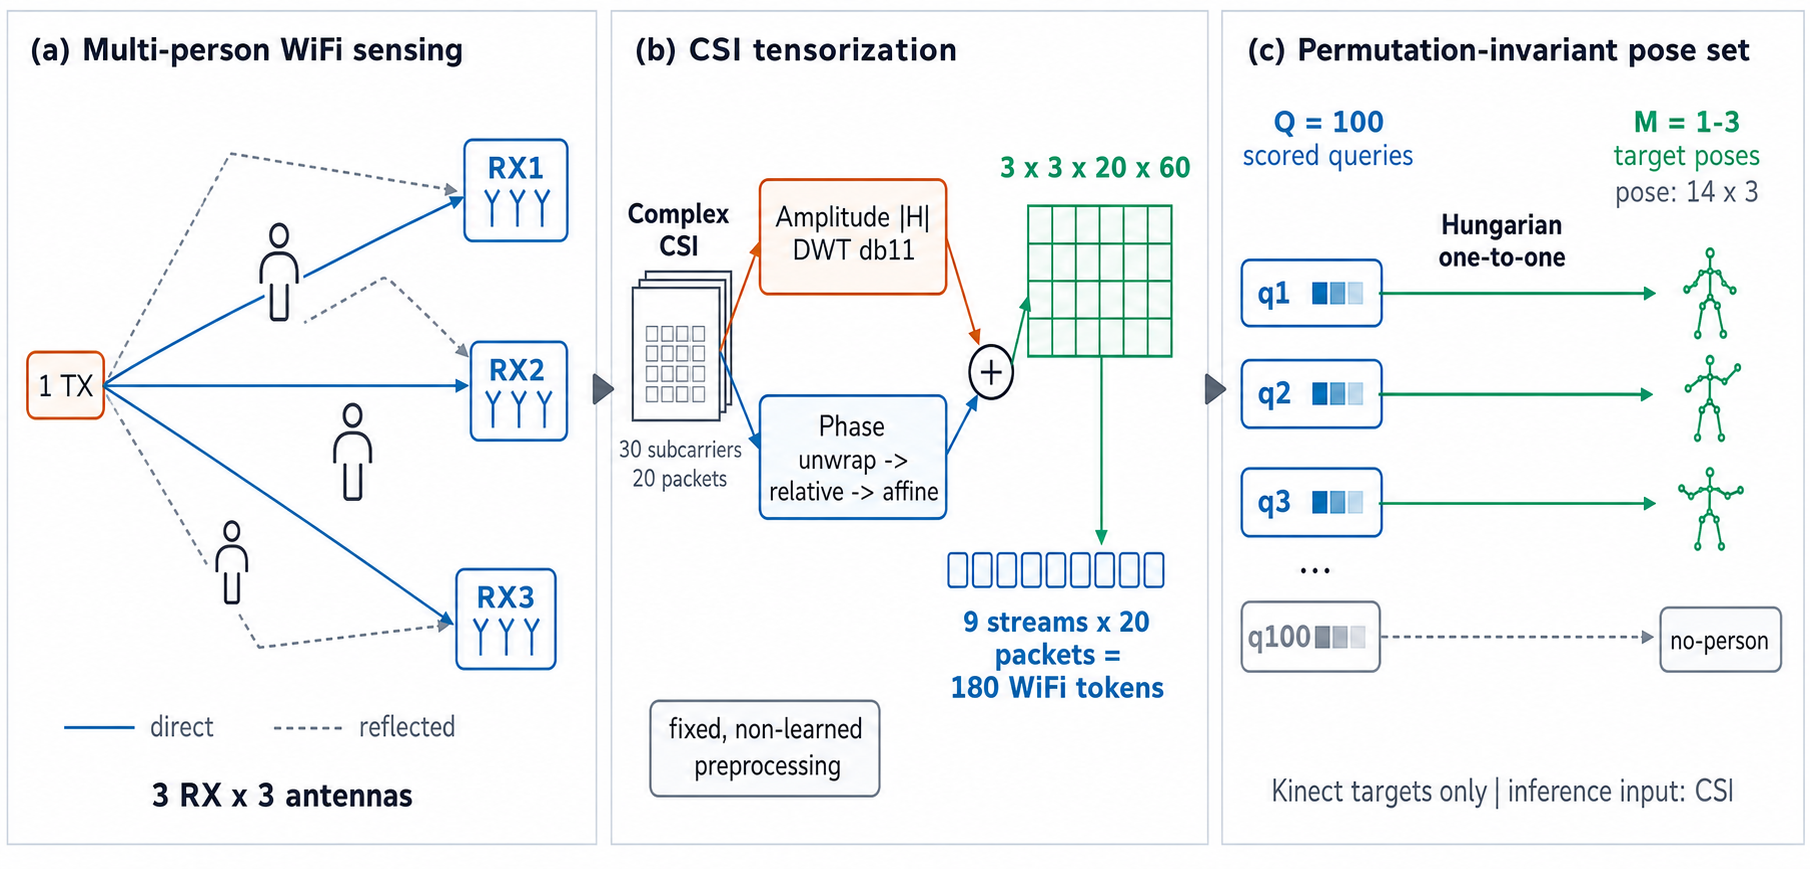
\includegraphics[width=0.85\textwidth]{figures/fig_problem_formulation_gpt_final.png}
    \caption{Sensing-to-set formulation (not to scale). (a) One transmitter and three three-antenna receivers observe direct and reflected paths perturbed by multiple people. (b) Fixed amplitude and phase preprocessing converts a 30-subcarrier, 20-packet CSI window into a $3\times3\times20\times60$ tensor; its $9\times20$ sequence positions yield 180 WiFi tokens. (c) Hungarian assignment matches $Q{=}100$ scored queries one-to-one to $M\in\{1,2,3\}$ target poses in $\mathbb R^{14\times3}$; unmatched queries learn no-person. Kinect supplies training targets only, whereas CSI is the inference input.}
    \label{fig:problem-formulation}
\end{figure*}

\subsection{CSI Preprocessing and Phase Calibration}
The raw amplitude and phase require deterministic conditioning before tensor construction. For amplitude, we apply DWT-based amplitude preprocessing: each $|H_i|$ sequence is decomposed with the \texttt{db11} wavelet under symmetric boundary handling and reconstructed at its original length. This operation regularizes the representation without introducing learned parameters. For phase, we first unwrap the reference-antenna phase, express the other antennas through successive relative phases, and estimate a common affine component over subcarrier index. Removing that component reduces packet-dependent linear phase distortion while retaining inter-antenna structure, following the calibration principle used by PhaseFi \cite{wang2015phasefi}. Figure~\ref{fig:problem-formulation}(b) emphasizes that both branches are fixed preprocessing; neither is optimized with the pose network.

\subsection{Sensing Layout and Tensor Construction}
The fixed-layout acquisition uses $1$ transmitter $\times$ $3$ receivers $\times$ $3$ antennas $\times$ $30$ active subcarriers $\times$ $20$ packets, giving a raw window of size $1\times3\times3\times30\times20$. For each receiver--antenna stream, the 30 amplitude values and 30 calibrated phase values are concatenated into 60 features. Dropping the singleton transmitter axis and transposing the remaining axes produces
\begin{equation}
    X\in\mathbb R^{3\times3\times20\times60}.
    \label{eq:csi-tensor}
\end{equation}
The nine receiver--antenna streams combined with 20 packet positions yield $9\times20=180$ WiFi tokens for the encoder. This ordering preserves spatial stream identity and short temporal context while making the model interface explicit. Kinect supplies synchronized ground-truth poses during data collection and training supervision; it is not an input at inference. Section~\ref{sec:dataset-acquisition} describes the acquisition protocol.

\subsection{Multi-Person 3D Pose Formulation}
For one CSI window, let the unordered ground-truth pose set be $\mathcal P=\{p_m\}_{m=1}^{M}$, where $p_m\in\mathbb R^{14\times3}$ and $M\in\{1,2,3\}$. The model emits $Q=100$ scored predictions
\begin{equation}
    \hat{\mathcal P}=\{(\hat p_q,s_q)\}_{q=1}^{Q},
    \qquad \hat p_q\in\mathbb R^{14\times3},\quad s_q\in[0,1].
    \label{eq:predicted-pose-set}
\end{equation}
Because person order has no semantic meaning, supervision is permutation-invariant. Let $\Pi_{M,Q}$ denote the injective mappings from the $M$ targets to the $Q$ queries. Hungarian assignment selects
\begin{equation}
    \pi^{*}=\arg\min_{\pi\in\Pi_{M,Q}}
    \sum_{m=1}^{M}\mathcal C\!\left((\hat p_{\pi(m)},s_{\pi(m)}),p_m\right),
    \label{eq:hungarian-task}
\end{equation}
where $\mathcal C$ combines person classification and pose-coordinate costs. As shown in Fig.~\ref{fig:problem-formulation}(c), matched queries receive pose and person supervision, whereas unmatched queries learn the no-person class. At inference, the scored queries form a score-ranked pose set without requiring Kinect input. Section~\ref{sec:eval-metrics} defines the localization and missed-person metrics used to evaluate this set-valued output.

\FloatBarrier

\section{Method}
\label{sec:method}
\subsection{Overview}
Figure~\ref{fig:system} summarizes the complete draft-to-refine path. A preprocessed CSI tensor is converted into 180 WiFi tokens, encoded by a compact sequence model, decoded into person hypotheses, and refined from draft pose to final pose through a conditional flow module. Table~\ref{tab:notation} fixes the tensor notation used throughout this section. The design deliberately separates representation, sequence modeling, query-based pose decoding, and refinement so that the controlled comparisons in Tables~\ref{tab:variant-summary}--\ref{tab:flow} isolate their respective effects.

\begin{figure}[t]
    \centering
    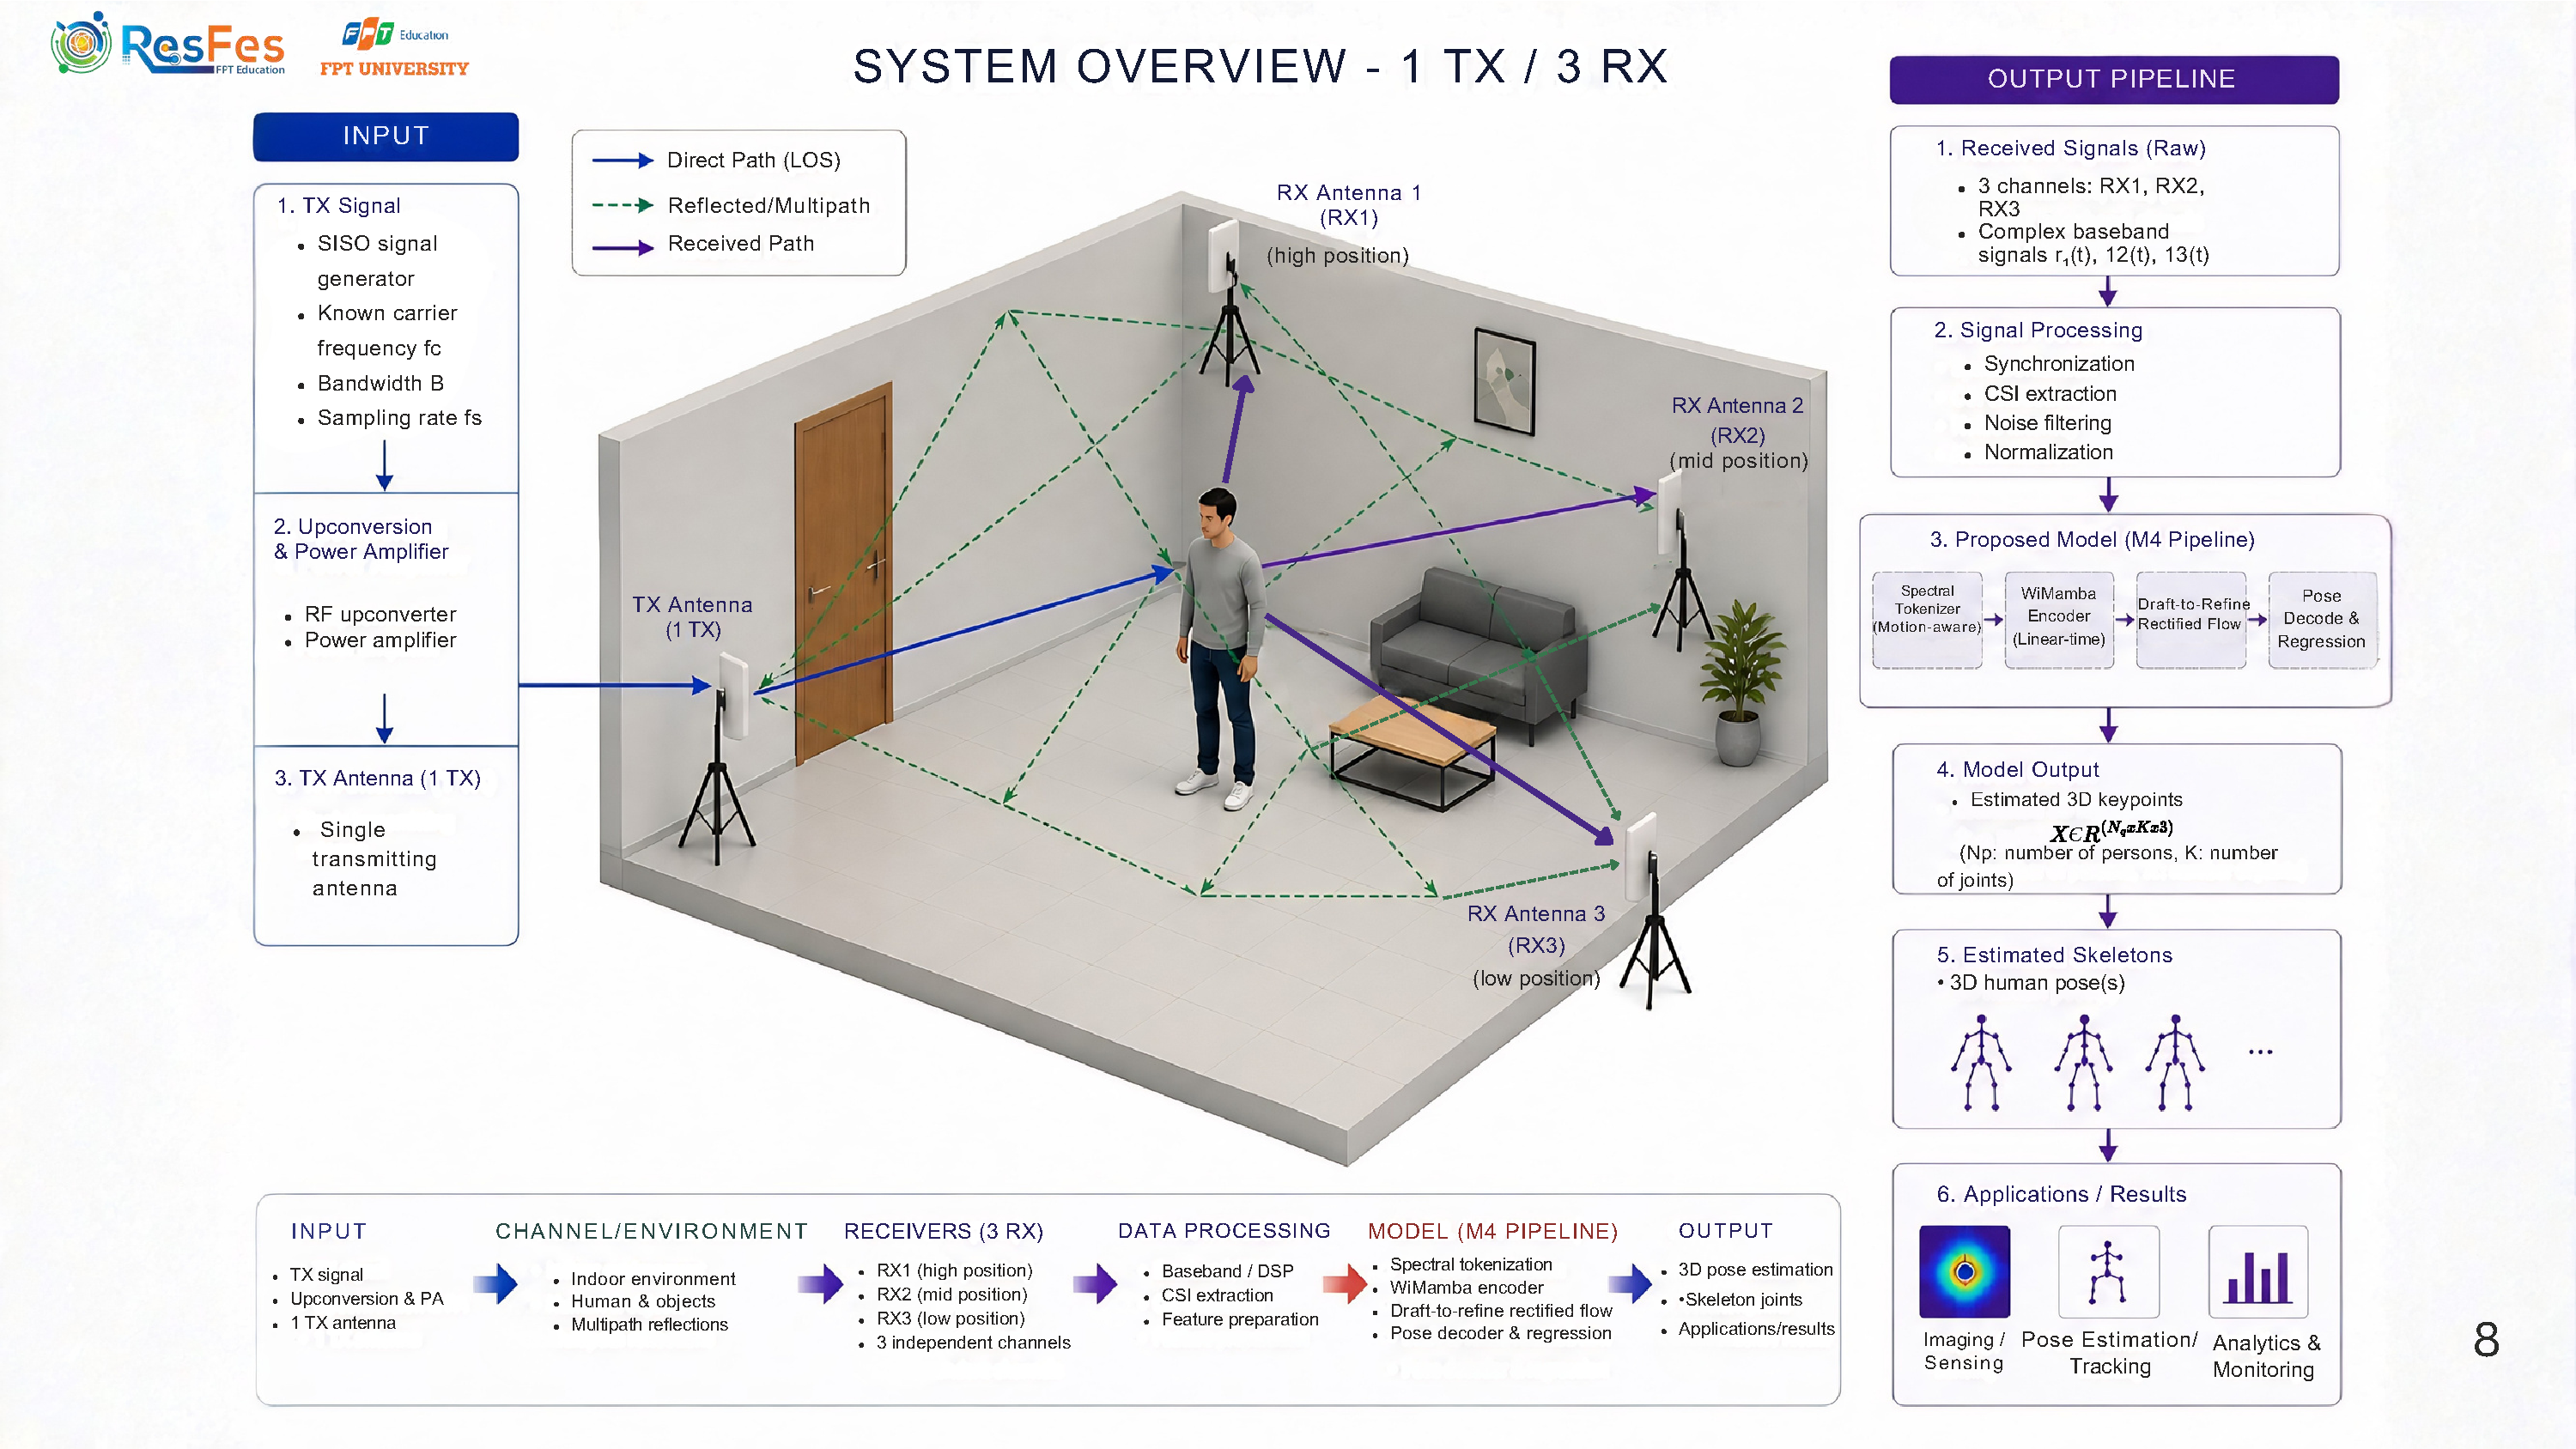
\includegraphics[width=0.98\linewidth]{figures/fig_system_overview.pdf}
\caption{System overview of the compact draft-to-refine pipeline under the fixed three-receiver protocol. The $3\times3\times20\times60$ CSI tensor is mapped to 180 256-D tokens, processed by the flattened Mamba-2 encoder, decoded by 100 learned queries, and refined in 42-D pose space by two Euler steps.}
    \label{fig:system}
\end{figure}

\begin{table}[H]
\centering
\caption{Notation and tensor shapes for the selected Mamba-2 Flow (two steps) configuration. $B$ is batch size and $Q{=}100$ is the number of learned pose queries.}
\label{tab:notation}
\begin{tabular}{l l l}
\toprule
Symbol & Shape & Meaning \\
\midrule
$X$ & $B\times3\times3\times20\times60$ & Preprocessed CSI tensor \\
$Z$ & $B\times180\times256$ & Linear CSI tokens, arranged as $9\times20$ \\
$H$ & $B\times180\times256$ & Flattened Mamba-2 encoded tokens \\
$q$ & $B\times Q\times256$ & Query features after cross-attention \\
$\hat p, p$ & $B\times Q\times42$ & Draft and ground-truth 14-keypoint poses \\
$c$ & $B\times Q\times256$ & Query condition for flow refinement \\
\bottomrule
\end{tabular}
\end{table}

\subsection{Spectrally Conditioned Temporal Residual Tokenization}
The control-path linear projection maps every 60-dimensional amplitude--phase CSI feature to a 256-dimensional token,
\begin{equation}
Z=W_{\mathrm{in}}X+b,\qquad Z\in\mathbb{R}^{B\times180\times256}.
\label{eq:token-proj}
\end{equation}
The Spectral Tokenizer retains this projection as a residual bypass and reshapes $Z$ as $Z^{\mathrm{grid}}\in\mathbb R^{B\times9\times20\times256}$. Each of the nine receiver--antenna links is processed independently. First, a depthwise temporal convolution with kernel size 5 and GELU activation extracts local temporal features,
\begin{equation}
\tilde Z_{b,s,:,:}=\operatorname{GELU}\!\left(
\operatorname{DWConv1D}(Z^{\mathrm{grid}}_{b,s,:,:})\right).
\label{eq:token-conv}
\end{equation}
Second, a 20-point orthonormal real FFT is applied to the projected tokens $Z^{\mathrm{grid}}$, yielding 11 nonredundant bins. Magnitudes are averaged over the 256 projected channels to produce a one-sided projected-feature spectral descriptor for link $s$,
\begin{equation}
d_{b,s,f}=\frac{1}{256}\sum_{c=1}^{256}
\left|\operatorname{RFFT}_{t}\!\left(Z^{\mathrm{grid}}_{b,s,t,c}\right)_f\right|,
\quad d_{b,s,:}\in\mathbb R^{11}.
\label{eq:token-gate}
\end{equation}
A two-layer MLP with dimensions $11\rightarrow22\rightarrow20$ and a sigmoid then produces a separate spectrally conditioned temporal gate $g_{b,s,:}$ for each link,
\begin{equation}
g_{b,s,:}=\sigma\!\left(\operatorname{MLP}_{11\rightarrow22\rightarrow20}
(d_{b,s,:})\right)\in(0,1)^{20}.
\label{eq:token-temporal-gate}
\end{equation}
Finally, the gate modulates the local temporal branch. A channel projection $W_c$ maps the branch back to the token space before residual addition and LayerNorm,
\begin{equation}
Z_{\mathrm{spec}}=\operatorname{LN}\!\left(Z+W_c\big(g\odot\tilde Z\big)\right).
\label{eq:token-fusion}
\end{equation}
$W_c$ is zero-initialized, making the residual correction exactly zero at initialization. This zero-initialized residual correction means that spectral mode begins at $\operatorname{LN}(Z)$, rather than at the unnormalized linear control $Z$. The tokenizer uses a compact projected-feature spectral descriptor to condition a per-link temporal residual update; it is not a calibrated velocity estimator, and the learned gate is not itself evidence that a particular time step corresponds to physical motion.

Figure~\ref{fig:spectral-tokenizer} exposes the residual bypass, temporal branch, descriptor computation, and link-specific gate separately. This decomposition also motivates the component controls used for tokenizer diagnostics: linear projection, projection plus LayerNorm, temporal residual without spectral conditioning, spectral gate over projected tokens without temporal convolution, and the full temporal--spectral residual composition. These diagnostics retain the Transformer-PETR control encoder and head so that tokenizer components are not conflated with later Mamba or pose-head changes.

\begin{figure}[!t]
    \centering
    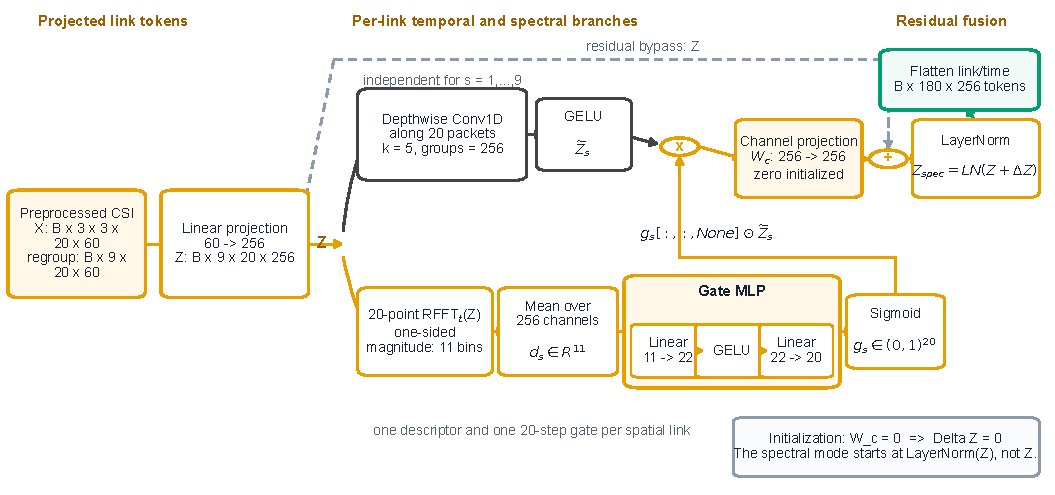
\includegraphics[width=0.99\linewidth]{figures/fig_spectral_tokenizer.pdf}
    \caption{Spectrally conditioned temporal residual tokenization. Projected CSI features are regrouped into nine 20-packet link sequences. For each link, a depthwise temporal branch is modulated by a 20-step gate computed from the 11-bin one-sided magnitude descriptor of the projected tokens. The gated features pass through a zero-initialized channel projection and are added to the projected-token bypass before LayerNorm; the resulting $9\times20$ grid is flattened to 180 tokens. At initialization, the correction is zero and the spectral mode returns $\operatorname{LayerNorm}(Z)$.}
    \label{fig:spectral-tokenizer}
\end{figure}

\subsection{Flattened Mamba-2 Sequence Encoder}
The flattened Mamba-2 sequence encoder replaces the Transformer-heavy sequence path with a time-major sequence of length 180. For layer $\ell$, the implementation performs pre-normalization, one Mamba-2 block, dropout, and a residual update,
\begin{equation}
H^{\ell+1}=H^\ell+\operatorname{Dropout}\!\left(
\operatorname{Mamba2}\!\left(\operatorname{LN}(H^\ell)\right)\right).
\label{eq:mamba-block}
\end{equation}
The selected encoder stacks three such blocks with embedding dimension 256, $d_{\mathrm{state}}{=}64$, $d_{\mathrm{conv}}{=}4$, expansion 2, head dimension 64, and dropout 0.1. Tokens are traversed in time-major order, without positional embeddings, spatial-attention premixing, or a final attention block. Equation~\ref{eq:mamba-block} describes the instantiated residual computation rather than introducing an additional generic state-space approximation. The motivation and original Mamba-2 formulation are given by \cite{dao2024mamba2}.

\subsection{Lightweight Query-Pose Head and Flow Refinement}
The lightweight query-pose head uses 100 learned queries and 8-head cross-attention to summarize the encoded CSI sequence. A two-hidden-layer MLP predicts a 42-dimensional draft pose, corresponding to 14 three-dimensional keypoints, and a binary classifier assigns each query a person score. Hungarian matching identifies positive queries; classification, keypoint, and bone losses are evaluated on these draft predictions using the shared set-prediction objective \cite{yan2024personwifi3d,shi2022petr}.

For each matched positive, the flow module receives the detached draft pose, target pose, and 256-dimensional query condition. The starting point and straight interpolation path are
\begin{equation}
x_0=\operatorname{stopgrad}(\hat p_{\mathrm{draft}})+\epsilon,\quad
\epsilon\sim\mathcal{N}(0,0.1^2),\quad t\sim U[0,1],
\label{eq:flow-start}
\end{equation}
\begin{equation}
x_t = (1-t)x_0 + t x_1,
\label{eq:flow-path}
\end{equation}
\begin{equation}
v^*(x_t,t,c)=x_1-x_0,
\label{eq:flow-target}
\end{equation}
\begin{equation}
\mathcal{L}_{\mathrm{flow}}=\operatorname{mean}\left\|v_\theta(x_t,t,c)-v^*(x_t,t,c)\right\|_2^2.
\label{eq:flow-loss}
\end{equation}
The conditional velocity network concatenates the 42-dimensional pose, the 256-dimensional query condition, and a 64-dimensional sinusoidal time embedding. It projects the resulting 362-dimensional vector to 512 dimensions, applies three residual MLP blocks, and predicts a 42-dimensional velocity. At inference, Euler integration updates the pose for $N\in\{1,2\}$ steps with $\Delta t=1/N$:
\begin{equation}
x_{k+1}=x_k+\Delta t\,v_\theta(x_k,t_k,c),\qquad t_k=k/N.
\label{eq:euler}
\end{equation}
Thus, the one-step and two-step settings use $\Delta t=1$ and $\Delta t=0.5$, respectively, to report final 3D keypoints. Figure~\ref{fig:flow} depicts this conditional draft-to-refine trajectory and the two-step Euler path used by the selected accuracy-oriented configuration. Algorithm~\ref{alg:draft-to-refine} consolidates the shared CSI-to-draft forward pass, matched-positive flow training, and score-ranked Euler inference.

\begin{algorithm}[!t]
\caption{Conditional draft-to-refine pose estimation}
\label{alg:draft-to-refine}
\begin{algorithmic}[1]
\REQUIRE Preprocessed CSI $X$; mode $m$; ground-truth pose set $\mathcal G$ if training; Euler steps $N\in\{1,2\}$ if testing.
\ENSURE Training loss $\mathcal L$, or score-ranked refined pose set $\mathcal R$.
\STATE \textbf{Shared forward pass}
\STATE Form spectrally conditioned residual tokens $Z_{\mathrm{spec}}\in\mathbb R^{B\times180\times256}$ by Equations~\ref{eq:token-proj}--\ref{eq:token-fusion}.
\STATE Encode the time-major token sequence with three residual Mamba-2 blocks (Equation~\ref{eq:mamba-block}) to obtain $H$.
\STATE Cross-attend $Q{=}100$ learned person queries to $H$ to obtain query features $q$; set flow conditions $c\leftarrow q$.
\STATE Predict draft coordinates $\hat p\in\mathbb R^{B\times Q\times42}$ and person scores $s$ from $q$.
\IF{$m=\mathrm{train}$}
    \STATE \textbf{Training branch}
    \STATE Apply Hungarian assignment to $(s,\hat p)$ and $\mathcal G$; let $\mathcal M$ contain the matched query--target pairs $(i,j)$.
    \STATE Compute $\mathcal L_{\mathrm{cls}}$ over all queries and $\mathcal L_{\mathrm{kpt}},\mathcal L_{\mathrm{bone}}$ over pairs in $\mathcal M$.
    \FOR{each matched pair $(i,j)\in\mathcal M$}
        \STATE Set $x_1\leftarrow p_j$ and sample $x_0\leftarrow\operatorname{stopgrad}(\hat p_i)+\epsilon$ by Equation~\ref{eq:flow-start}.
        \STATE Sample $t\sim U[0,1]$ and form $x_t\leftarrow(1-t)x_0+t x_1$ by Equation~\ref{eq:flow-path}.
        \STATE Set target velocity $v^*\leftarrow x_1-x_0$ (Equation~\ref{eq:flow-target}) and predict $v_\theta(x_t,t,c_i)$.
    \ENDFOR
    \STATE Average the velocity MSE over $\mathcal M$ to obtain $\mathcal{L}_{\mathrm{flow}}$ in Equation~\ref{eq:flow-loss}; use zero if $\mathcal M=\varnothing$.
    \STATE $\mathcal{L}=2\mathcal{L}_{\mathrm{cls}}+5\mathcal{L}_{\mathrm{kpt}}+2\mathcal{L}_{\mathrm{bone}}+10\mathcal{L}_{\mathrm{flow}}$.
    \STATE \textbf{return} $\mathcal L$.
\ELSE
    \STATE \textbf{Inference branch}
    \STATE Rank the $Q$ queries by $s$ and retain indices $\mathcal I$ (all $Q{=}100$ under the reported protocol).
    \STATE Initialize $x\leftarrow\hat p_{\mathcal I}$, $c\leftarrow q_{\mathcal I}$, and $\Delta t=1/N$.
    \FOR{$k=0,\ldots,N-1$}
        \STATE Set $t_k\leftarrow k/N$ and update $x\leftarrow x+\Delta t\,v_\theta(x,t_k,c)$ by Equation~\ref{eq:euler}.
    \ENDFOR
    \STATE Reshape each row of $x$ to $14\times3$ keypoints and return $\mathcal R=\{(x_i,s_i):i\in\mathcal I\}$.
\ENDIF
\end{algorithmic}
\end{algorithm}

\subsection{Implementation Details}
The selected Mamba-2 Flow (two steps) configuration uses 100 learned person queries, 256-dimensional embeddings, and 14 output keypoints. The Spectrally Conditioned Temporal Residual Tokenizer maps the CSI tensor to a flattened sequence; its gate MLP is $11\rightarrow22\rightarrow20$, and its residual channel projection is zero-initialized. The three-layer Mamba-2 encoder uses $d_{\mathrm{state}}{=}64$, $d_{\mathrm{conv}}{=}4$, expansion 2, head dimension 64, dropout 0.1, and time-major token ordering; it does not add positional embeddings or a final attention block. The lightweight query-pose head applies 8-head query attention, a two-layer MLP draft regressor, and a binary classification head. Refinement uses a conditional MLP velocity field over 3D keypoint coordinates, integration time, and query-level features.

Training uses the weighted objective $\mathcal L=2.0\mathcal L_{\mathrm{cls}}+5.0\mathcal L_{\mathrm{kpt}}+2.0\mathcal L_{\mathrm{bone}}+10.0\mathcal L_{\mathrm{flow}}$ for flow-refined variants; the last term is omitted when refinement is disabled. All configurations use AdamW with learning rate $2{\times}10^{-5}$ and weight decay $10^{-4}$. The set-prediction evaluation and its 500\,mm matching rule are formalized in Section~\ref{sec:eval-metrics}.

\begin{figure}[!t]
    \centering
    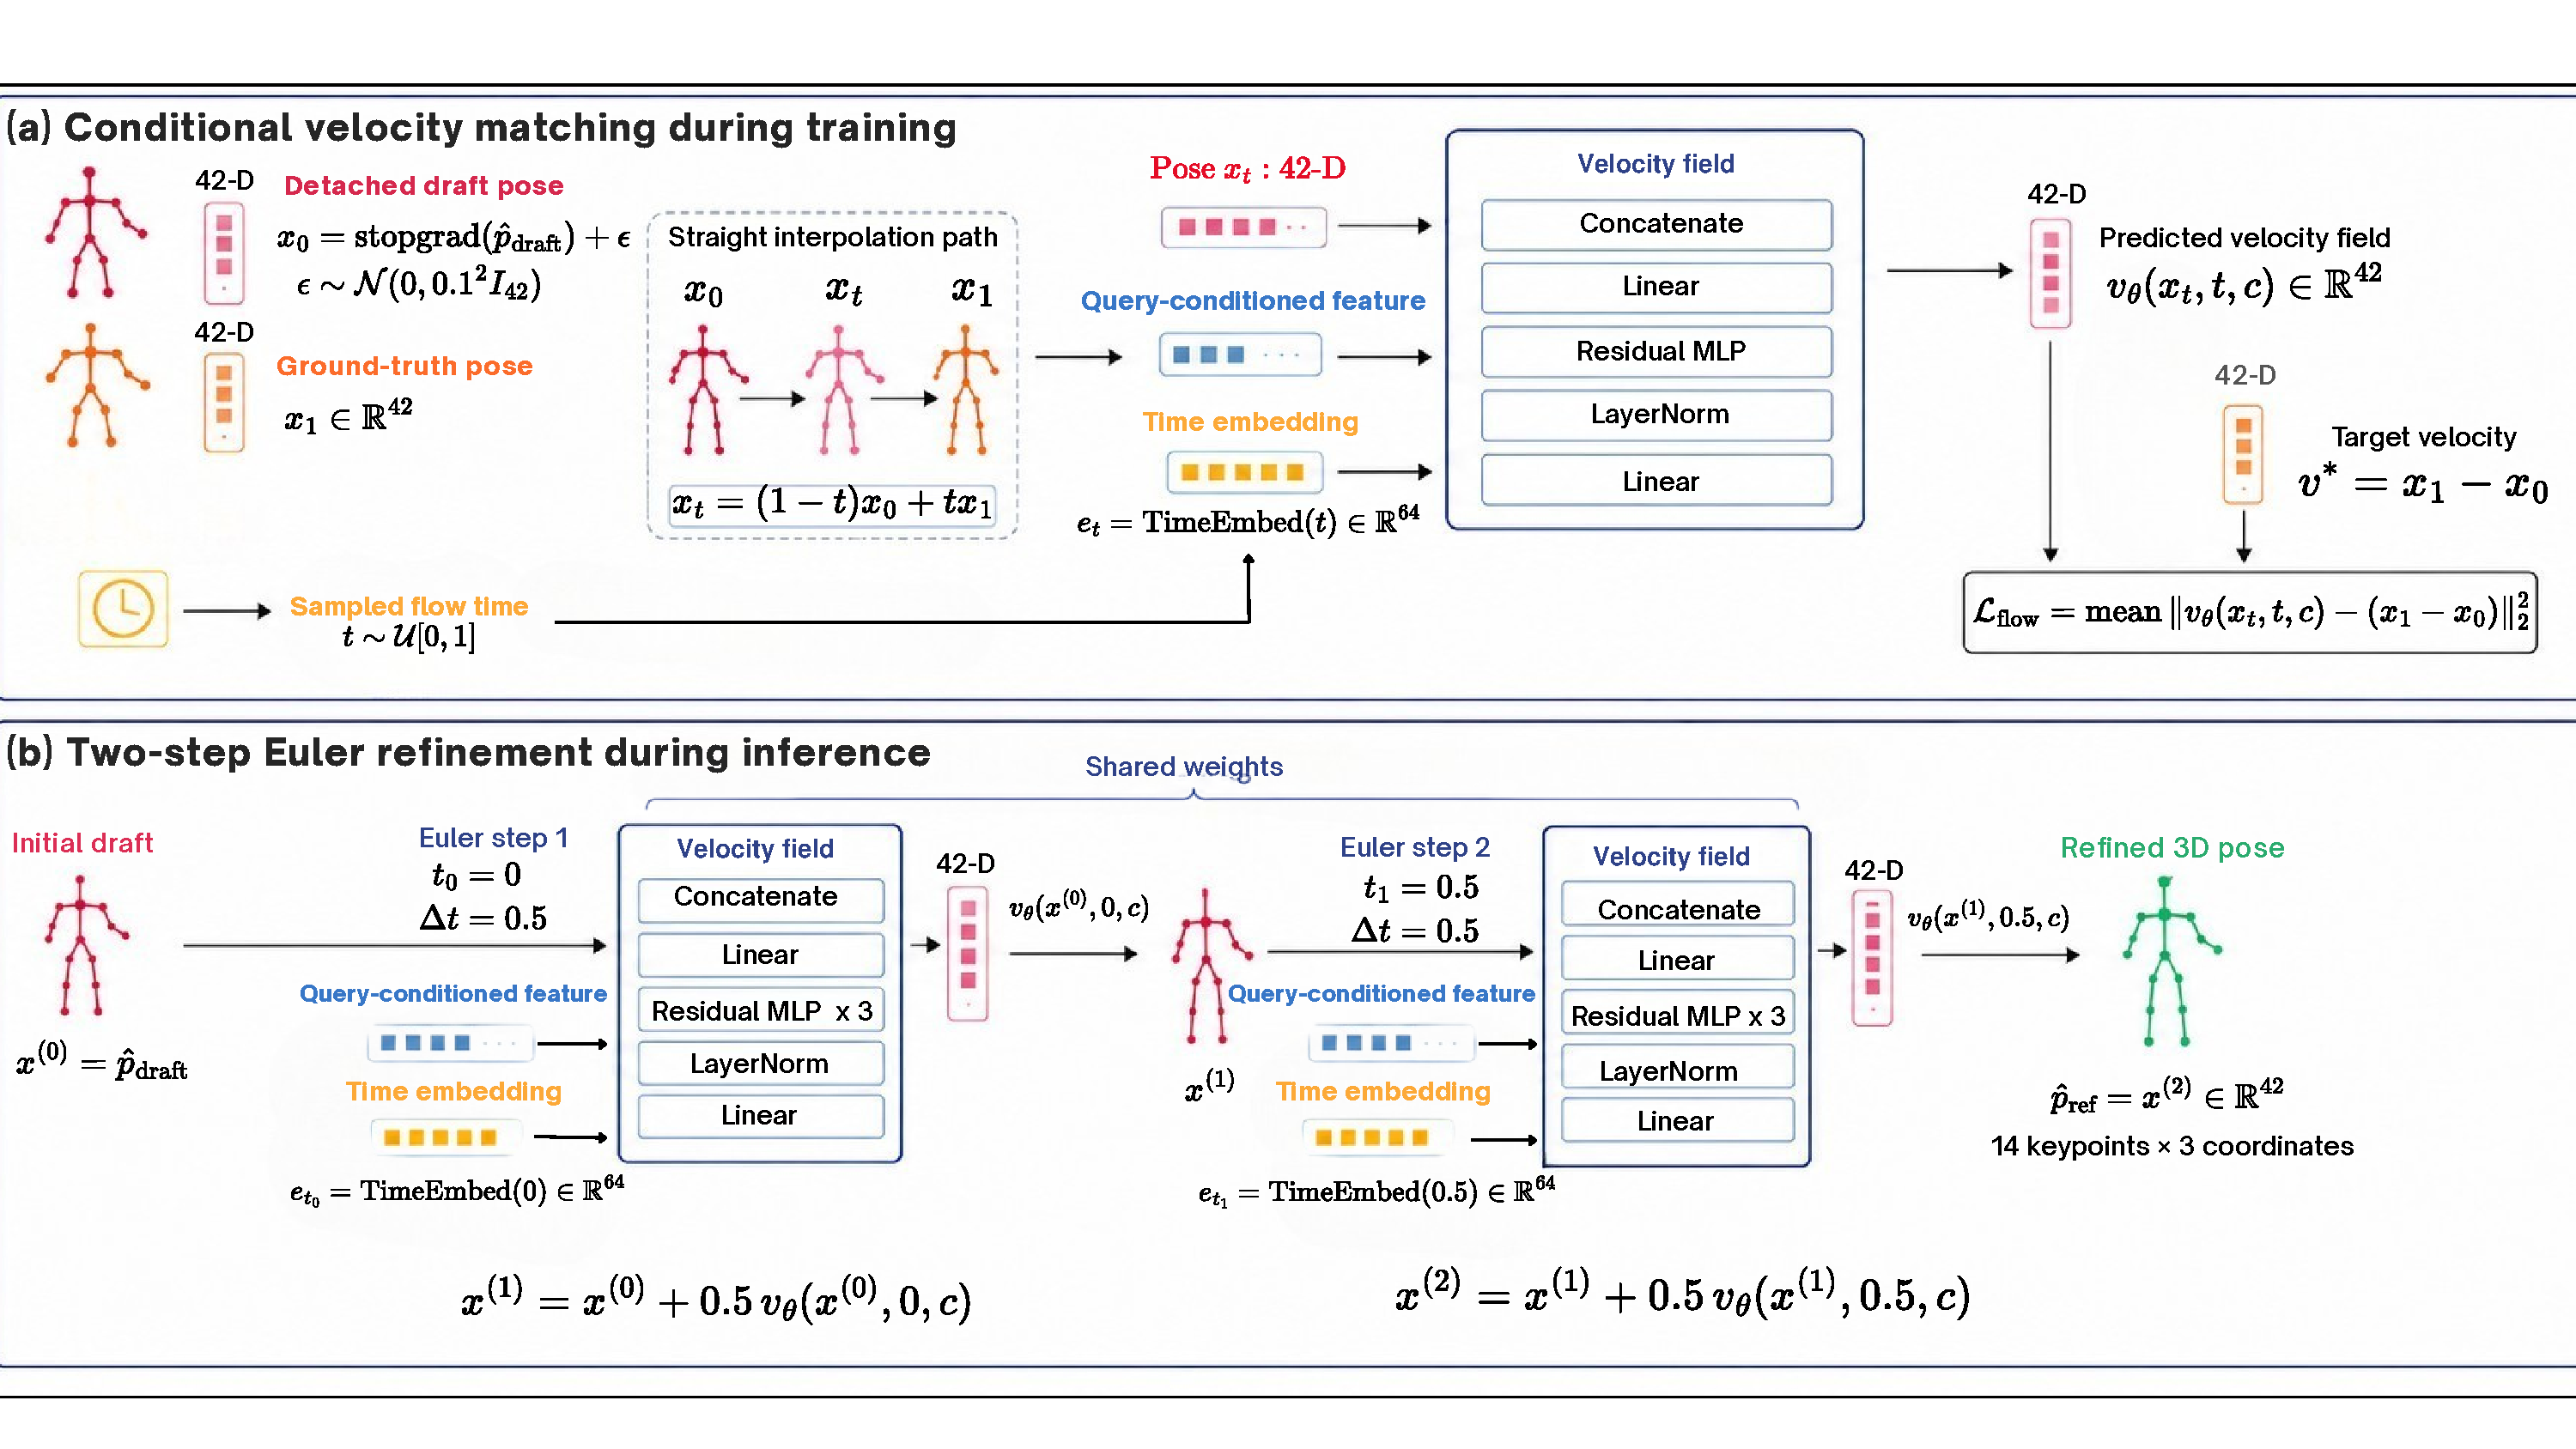
\includegraphics[width=0.95\linewidth]{figures/fig_flow_refinement_architecture.pdf}
    \caption{Conditional pose-flow refinement from 42-D draft coordinates to refined 3D keypoints. A matched query feature provides the 256-D condition $c$; training samples $t\sim U[0,1]$ along the path in Equation~\ref{eq:flow-path}, while the selected model applies two Euler updates from Equation~\ref{eq:euler} at inference.}
    \label{fig:flow}
\end{figure}

\section{Experimental Methodology}
\subsection{Dataset and Acquisition}
\label{sec:dataset-acquisition}
We use the public fixed-layout CSI--RGB-D benchmark and acquisition protocol released with \cite{yan2024personwifi3d}. The benchmark release reports ethics clearance for public reuse; this study collects no additional participant data. Four ThinkPad X201 laptops equipped with Intel 5300 WiFi adapters form one transmitter and three receivers. The transmitter operates on channel 128 at 5.64~GHz through a single antenna, while each receiver records three antenna streams. It sends 300 packets per second and retains 30 subcarriers per transmitter--receiver link. An Azure Kinect captures synchronized RGB-D observations at 15 frames per second. Each CSI block has size $1 \times 3 \times 3 \times 30 \times 20$ for transmitter, receiver, antenna, subcarrier, and time; concatenating amplitude with sanitized phase, removing the singleton transmitter axis, and reordering axes yields the $3 \times 3 \times 20 \times 60$ input and 180 tokens.

The dataset contains recordings from seven volunteers performing eight daily actions across an office, classroom, and corridor. Under the published temporal split, each 40-second clip contributes its first 550 frames to training and final 50 frames to testing. Kinect SDK failures, including four-person cases, are excluded in the released benchmark; the resulting 1P/2P/3P split contains 89{,}946 training and 7{,}824 test samples, summarized in Table~\ref{tab:dataset-stats}.

\begin{table}[htbp]
\caption{Dataset statistics for the Person-in-WiFi 3D internal test bed
used throughout this paper. Counts are CSI samples; each sample is paired
with a synchronized Azure Kinect skeleton.}
\label{tab:dataset-stats}
\centering
\begin{tabular}{l r r r r}
\toprule
split & 1-person & 2-person & 3-person & total \\
\midrule
training & 28{,}121 & 36{,}242 & 25{,}583 & 89{,}946 \\
test     & 2{,}586  & 3{,}184  & 2{,}054  & 7{,}824  \\
\midrule
total    & 30{,}707 & 39{,}426 & 27{,}637 & 97{,}770 \\
\bottomrule
\end{tabular}
\end{table}


\subsection{Training Setup}
\label{sec:training-setup}
All configurations use the same 20-epoch AdamW schedule with base learning rate $2{\times}10^{-5}$, weight decay $10^{-4}$, batch size 32, deterministic seed 42, and FP32 precision. CSI inputs use discrete-wavelet amplitude denoising and phase normalization. Experiments run on an NVIDIA RTX 6000 Ada Generation GPU with PyTorch 2.1.0, CUDA 12.1, and cuDNN 8.9.2. Runtime is model-only \texttt{simple\_test} inference on a batch-one $3 \times 3 \times 20 \times 60$ tensor: preprocessing, data I/O, and evaluation matching are excluded. Each result uses 10 warm-up iterations followed by 100 synchronized FP32 measurements; latency is the mean, throughput its reciprocal, and memory is peak CUDA allocated memory.

\subsection{Research Questions}
The results are organized around three questions. RQ1 asks how representation, encoder, and compact pose-head choices affect the accuracy--efficiency trade-off. RQ2 asks how flow inference changes matched localization and missed-person behavior. RQ3 asks which configuration provides the most useful fixed-layout operating point under the shared protocol.

\subsection{Evaluation Metrics}
\label{sec:eval-metrics}
For a predicted 3D pose $\hat{P}$ and the matched ground truth $P_{gt}$, the per-joint position error (PJPE) of joint $k$ is the Euclidean distance between predicted and ground-truth coordinates. The mean per-joint position error (MPJPE) averages PJPE over the $K{=}14$ keypoints \cite{ionescu2014h36m}:
\begin{equation}
    \mathrm{PJPE}(k) = \left\| \hat{P}_k - P_{gt,k} \right\|_2,\quad
    \mathrm{MPJPE} = \frac{1}{K}\sum_{k=1}^{K} \mathrm{PJPE}(k).
\label{eq:mpjpe}
\end{equation}
To diagnose where error concentrates, we additionally report the per-joint dimension localization error (PJDLE), defined as the $\ell_1$ distance along each spatial axis $a \in \{h,v,d\}$:
\begin{equation}
    \mathrm{PJDLE}_a(k) = \left| \hat{P}_{k,a} - P_{gt,k,a} \right|,\quad
    \mathrm{MPJDLE}_a = \frac{1}{K}\sum_{k=1}^{K} \mathrm{PJDLE}_a(k).
\label{eq:mpjdle}
\end{equation}
Equations~\ref{eq:mpjpe} and~\ref{eq:mpjdle} use millimeters after the benchmark coordinate conversion.
For every frame, the 100 score-ranked queries are assigned to ground truth by Hungarian matching. Let $\mathcal M$ denote accepted pairs, $U$ the number of unmatched ground-truth persons, and $N_{\mathrm{GT}}=|\mathcal M|+U$ the number of ground-truth persons. Pairs whose person-level distance exceeds 500~mm are rejected. With the fixed benchmark miss penalty of 500~mm, the reported overall metric is
\begin{equation}
\operatorname{MPJPE}_{\mathrm{overall}}=
\frac{E_{\mathrm{matched}}+500\,U}{N_{\mathrm{GT}}},\qquad
E_{\mathrm{matched}}=\sum_{(\hat P,P)\in\mathcal M}\operatorname{MPJPE}(\hat P,P),
\label{eq:overall-mpjpe}
\end{equation}
whereas Matched MPJPE is $E_{\mathrm{matched}}/|\mathcal M|$. Overall MPJPE therefore combines matched-pose localization and missed-person coverage; it is not a detection average-precision metric. This shared benchmark metric is used consistently for every variant and is further separated by scene cardinality (1P/2P/3P) in Table~\ref{tab:main}.

\section{Results}
\subsection{Main Ablation}
RQ1 is answered by the full architecture ladder. Table~\ref{tab:variant-summary} maps stable experiment IDs to functional public names, while Table~\ref{tab:main} reports the corresponding accuracy and efficiency. The PETR variants vary the input and encoder; the draft variants introduce the lightweight query-pose head without refinement; and the flow variants add one- or two-step correction under Transformer, Mamba, and flattened Mamba-2 sequence encoders.

\begin{table}[!t]
\centering
\caption{Controlled architecture ladder. Experiment IDs provide stable links to benchmark artifacts; public labels describe the evaluated architecture.}
\label{tab:variant-summary}
\resizebox{\linewidth}{!}{%
\begin{tabular}{l l l l l l}
\toprule
Experiment ID & Input & Encoder & Pose Head & Refinement & Public label \\
\midrule
\modelid{modelM0}{M0} & Linear & Transformer & PETR query decoder & None & Transformer-PETR Control \\
\modelid{modelM1}{M1} & Spectral & Transformer & PETR query decoder & None & Spectral PETR \\
\modelid{modelM2}{M2} & Spectral & Mamba & PETR query decoder & None & Mamba PETR \\
\modelid{modelM3}{M3} & Spectral & Flattened Mamba-2 & PETR query decoder & None & Mamba-2 PETR \\
\modelid{modelM4}{M4} & Spectral & Transformer & Lightweight query-pose & None & Transformer Draft \\
\modelid{modelM5}{M5} & Spectral & Mamba & Lightweight query-pose & None & Mamba Draft \\
\modelid{modelM6}{M6} & Spectral & Flattened Mamba-2 & Lightweight query-pose & None & Mamba-2 Draft \\
\modelid{modelM7}{M7} & Spectral & Transformer & Lightweight query-pose & One step & Transformer Flow \\
\modelid{modelM8}{M8} & Spectral & Mamba & Lightweight query-pose & One step & Mamba Flow \\
\modelid{modelM9}{M9} & Spectral & Flattened Mamba-2 & Lightweight query-pose & One step & Mamba-2 Flow (1 step) \\
\modelid{modelM9RF2}{M9\_RF2} & Spectral & Flattened Mamba-2 & Lightweight query-pose & Two steps & Mamba-2 Flow (2 steps) \\
\bottomrule
\end{tabular}}
\end{table}

\begin{table}[!t]
\centering
\caption{Full 20-epoch ablation under the shared fixed-layout protocol. Lower MPJPE in millimeters, parameter count, and peak allocated memory are better; higher model-only batch-one FPS is better.}
\label{tab:main}
\resizebox{\linewidth}{!}{%
\begin{tabular}{l c c c c c c c}
\toprule
Experiment ID & MPJPE & 1P & 2P & 3P & FPS & Params (M) & Memory (MB) \\
\midrule
\modelid{modelM0}{M0} & 172.540 & 136.141 & 167.971 & 192.537 & 118.7 & 13.130 & 155.60 \\
\modelid{modelM1}{M1} & 169.271 & 132.597 & 163.323 & 190.810 & 83.1 & 13.199 & 155.86 \\
\modelid{modelM2}{M2} & 174.961 & 143.475 & 166.642 & 196.772 & 69.4 & 11.967 & 151.16 \\
\modelid{modelM3}{M3} & 175.658 & 140.116 & 169.358 & 197.084 & 102.0 & 10.292 & 142.69 \\
\modelid{modelM4}{M4} & 169.796 & 126.479 & 167.593 & 190.251 & 180.8 & 5.255 & 31.61 \\
\modelid{modelM5}{M5} & 171.055 & 127.258 & 171.979 & 188.481 & 116.8 & 4.023 & 26.80 \\
\modelid{modelM6}{M6} & 167.573 & 125.532 & 164.528 & \textbf{188.363} & \textbf{247.7} & \textbf{1.813} & \textbf{18.41} \\
\modelid{modelM7}{M7} & 168.342 & 127.129 & 162.775 & 191.390 & 145.8 & 7.059 & 38.49 \\
\modelid{modelM8}{M8} & 169.653 & 122.253 & 165.397 & 193.943 & 109.4 & 5.827 & 33.68 \\
\modelid{modelM9}{M9} & 168.086 & 125.958 & 161.832 & 192.229 & 206.9 & 3.618 & 25.29 \\
\modelid{modelM9RF2}{M9\_RF2} & \textbf{165.487} & \textbf{121.785} & \textbf{159.341} & 190.179 & 209.9 & 3.618 & 25.29 \\
\bottomrule
\end{tabular}}
\end{table}

Table~\ref{tab:main} shows that the lightweight query-pose path creates the largest efficiency shift in the ladder. Transformer Draft reaches 180.8 FPS with 5.255M parameters, while Mamba-2 Draft advances this compact design to 247.7 FPS, 1.813M parameters, and 18.41 MB peak allocated memory. This makes Mamba-2 Draft the throughput--memory endpoint and identifies the compact pose head as the setting in which flattened Mamba-2 provides its clearest efficiency benefit.

The encoder results also expose an architecture interaction. The full Spectral Tokenizer plus PETR reduces MPJPE from 172.540 to 169.271 mm relative to the linear Transformer-PETR Control, but this endpoint contrast does not isolate LayerNorm, temporal convolution, and spectral gating from one another. Substituting Mamba or Mamba-2 while retaining the heavier PETR head does not lower MPJPE. Once the lightweight query-pose head is introduced, the flattened Mamba-2 path reaches 167.573 mm and exceeds Transformer Draft by 2.223 mm MPJPE and 66.9 FPS. Encoder replacement alone is therefore insufficient; the benefit emerges from the compact encoder--head combination.

Mamba-2 Flow (two steps) is the accuracy-oriented endpoint. It achieves 165.487 mm MPJPE at 209.9 FPS with 3.618M parameters and 25.29 MB peak allocated memory. Relative to the Transformer-PETR Control, this is a 7.053 mm (4.09\%) MPJPE reduction, 1.77$\times$ higher throughput, 72.45\% fewer parameters, and 83.75\% lower peak allocated memory. Relative to Mamba-2 Draft, the flow endpoint exchanges 15.25\% throughput for a further 2.086 mm MPJPE reduction. The ladder therefore exposes two useful operating points rather than one undifferentiated ``best'' model (Table~\ref{tab:main} and Figure~\ref{fig:main_ablation}).

\begin{figure}[!t]
    \centering
    
\includegraphics[width=0.96\linewidth]{figures/fig_main_ablation_mpjpe_latency_params.pdf}
\caption{Accuracy and efficiency across the controlled architecture ladder in Table~\ref{tab:main}. Lower MPJPE in millimeters, parameter count, and peak allocated memory are better; higher model-only batch-one FPS is better. Functional labels are defined in Table~\ref{tab:variant-summary}; values use the shared fixed-layout protocol.}
    \label{fig:main_ablation}
\end{figure}

\IfFileExists{tables/tokenizer_component_ablation.tex}{%
\subsection{Tokenizer Component Diagnostic}
The endpoint comparison in Table~\ref{tab:main} treats the Spectral Tokenizer as one representation-level package. The component diagnostic is interpreted only after the linear and full-tokenizer endpoints reproduce the corresponding ladder results within 1 mm.
\input{tables/tokenizer_component_ablation.tex}
}{}

\subsection{Flow Solver Analysis}
RQ2 separates draft inference, refinement bypass, one-step refinement, and two-step refinement. Table~\ref{tab:flow} and Figure~\ref{fig:flow_ablation} expose both matched-pose localization and unmatched-person count. Relative to refinement bypass, two-step refinement reduces overall MPJPE by 2.245 mm MPJPE and Matched MPJPE by 2.033 mm, while missed persons decrease from $82\rightarrow72$. Relative to one-step refinement, it reduces overall MPJPE by 2.599 mm MPJPE and Matched MPJPE by 2.523 mm, while missed persons decrease from $76\rightarrow72$.

Mamba-2 Draft produces the fewest missed persons (54) and remains the throughput endpoint, whereas Mamba-2 Flow (two steps) obtains the lowest overall and matched-only MPJPE. The comparison therefore separates coverage-oriented and localization-oriented behavior under the same benchmark metric: the two-step solver is the accuracy-oriented inference setting for the Mamba-2 Flow configuration (Table~\ref{tab:flow} and Figure~\ref{fig:flow_ablation}).

\begin{table}[!t]
\centering
\caption{Flow-solver analysis under the same Mamba-2 draft-to-refine architecture. Lower overall MPJPE, Matched MPJPE, and missed-person count are better; MPJPE values are in millimeters and use the fixed 500 mm benchmark miss penalty.}
\label{tab:flow}
\resizebox{\linewidth}{!}{%
\begin{tabular}{l l c c c c c c}
\toprule
Experiment ID & Public setting & MPJPE & Matched & Missed & 1P & 2P & 3P \\
\midrule
\modelid{modelM6}{M6} & Mamba-2 Draft & 167.573 & 166.381 & \textbf{54} & 125.532 & 164.528 & 188.363 \\
\modelid{modelM9}{M9\_no\_flow} & Mamba-2 Flow (refinement bypassed) & 167.732 & 165.919 & 82 & 122.870 & 163.026 & 191.421 \\
\modelid{modelM9}{M9} & Mamba-2 Flow (1 step) & 168.086 & 166.409 & 76 & 125.958 & 161.832 & 192.229 \\
\modelid{modelM9RF2}{M9\_RF2} & Mamba-2 Flow (2 steps) & \textbf{165.487} & \textbf{163.886} & 72 & 121.785 & 159.341 & 190.179 \\
\bottomrule
\end{tabular}}
\end{table}

\begin{figure}[!t]
    \centering
    
\includegraphics[width=0.90\linewidth]{figures/fig_flow_solver_ablation.pdf}
\caption{Flow-solver analysis for the four settings in Table~\ref{tab:flow}. Lower values are better in both panels: (a) overall MPJPE in millimeters, including the fixed 500 mm penalty for unmatched ground-truth persons; and (b) unmatched ground-truth person count. The highlighted point denotes Mamba-2 Flow (2 steps).}
    \label{fig:flow_ablation}
\end{figure}

\subsection{Operating Point and Qualitative Cases}
\label{sec:failure-cases}
RQ3 asks which tested configuration provides the most useful fixed-layout operating point. Mamba-2 Draft is the efficiency endpoint, whereas Mamba-2 Flow (two steps) is the accuracy-oriented choice because it attains the lowest MPJPE while retaining 209.9 FPS. Figure~\ref{fig:qualitative} shows representative 1-person, 2-person, and 3-person samples for the Transformer-PETR Control, Transformer Flow, and Mamba-2 Flow (two steps). The panel footers provide sample-level matching diagnostics that make the pose overlays auditable; aggregate conclusions remain grounded in Tables~\ref{tab:main} and~\ref{tab:flow}, not in these selected examples.

\begin{figure}[t]
    \centering
    \IfFileExists{figures/fig_qualitative_full_paper.pdf}{%
        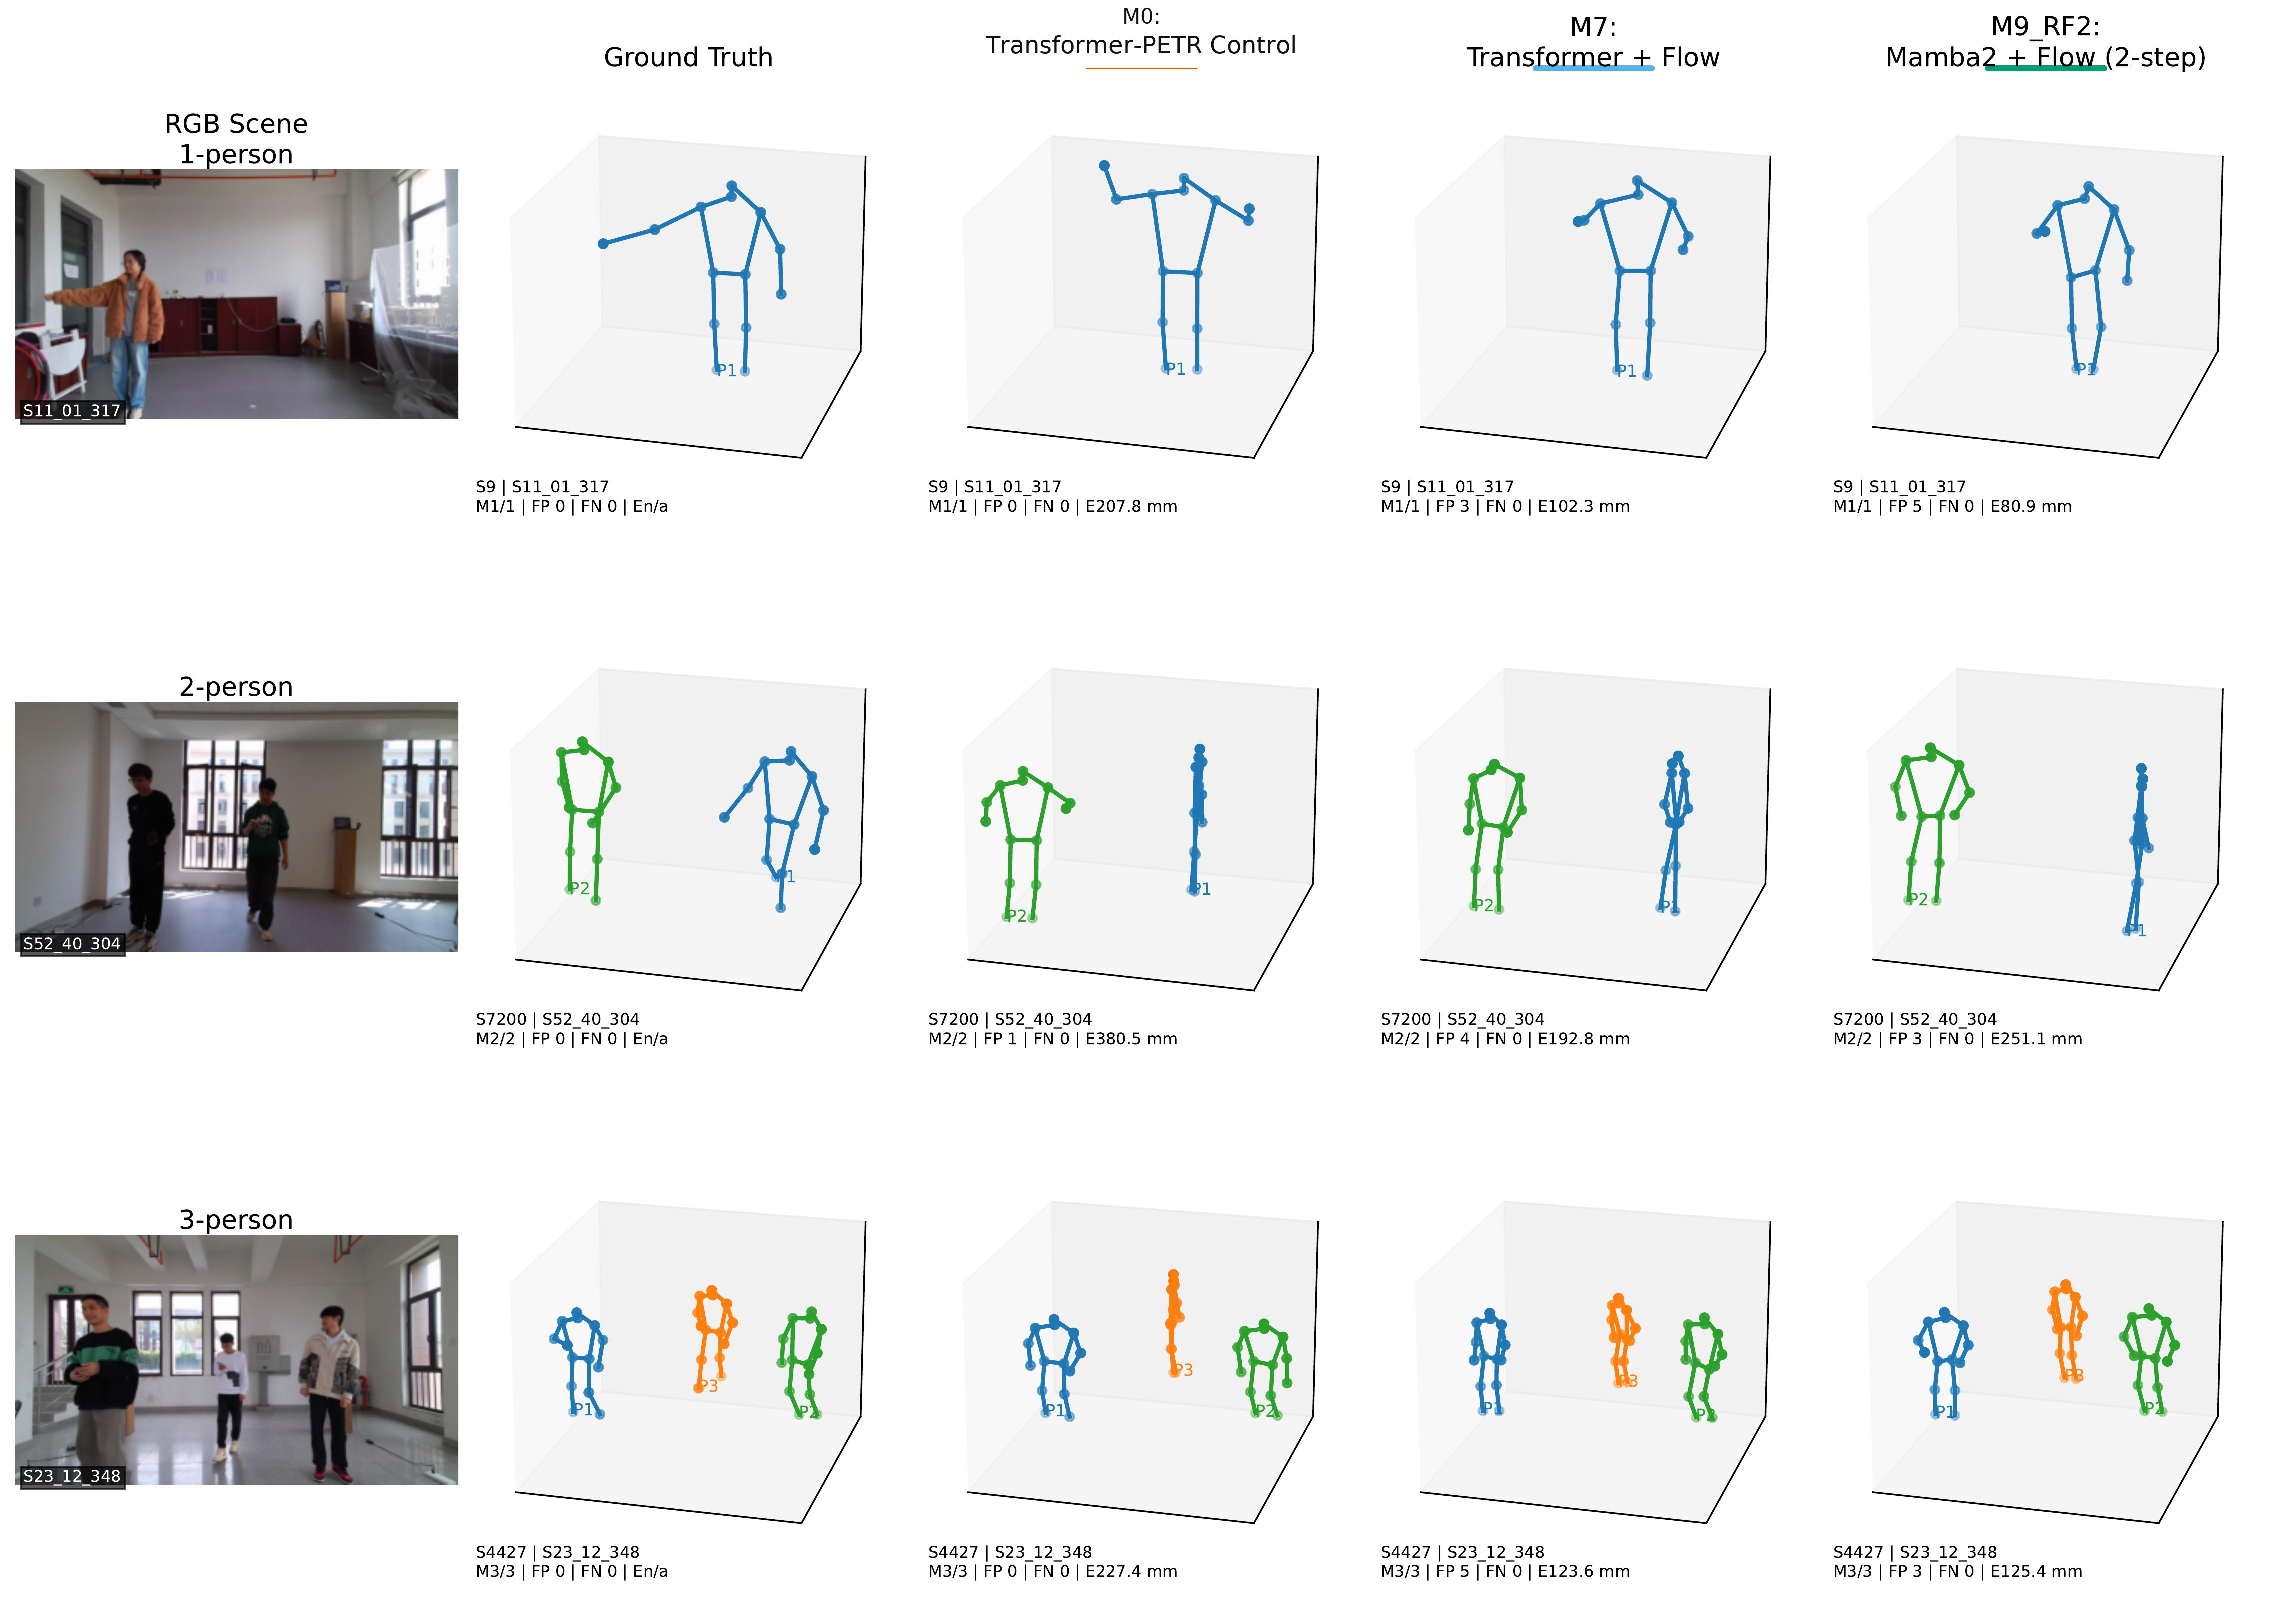
\includegraphics[width=0.99\linewidth]{figures/fig_qualitative_full_paper.pdf}
        \caption{Selected qualitative WiFi pose samples across 1-person, 2-person, and 3-person settings under the same held-out split as Tables~\ref{tab:main} and~\ref{tab:flow}. Columns show the synchronized RGB scene, Kinect ground truth, Transformer-PETR Control, Transformer Flow, and Mamba-2 Flow (two steps) predictions. Unmatched predictions above the fixed confidence threshold are gray. Panel footers report per-sample matching diagnostics rather than aggregate test metrics.}
    }{%
        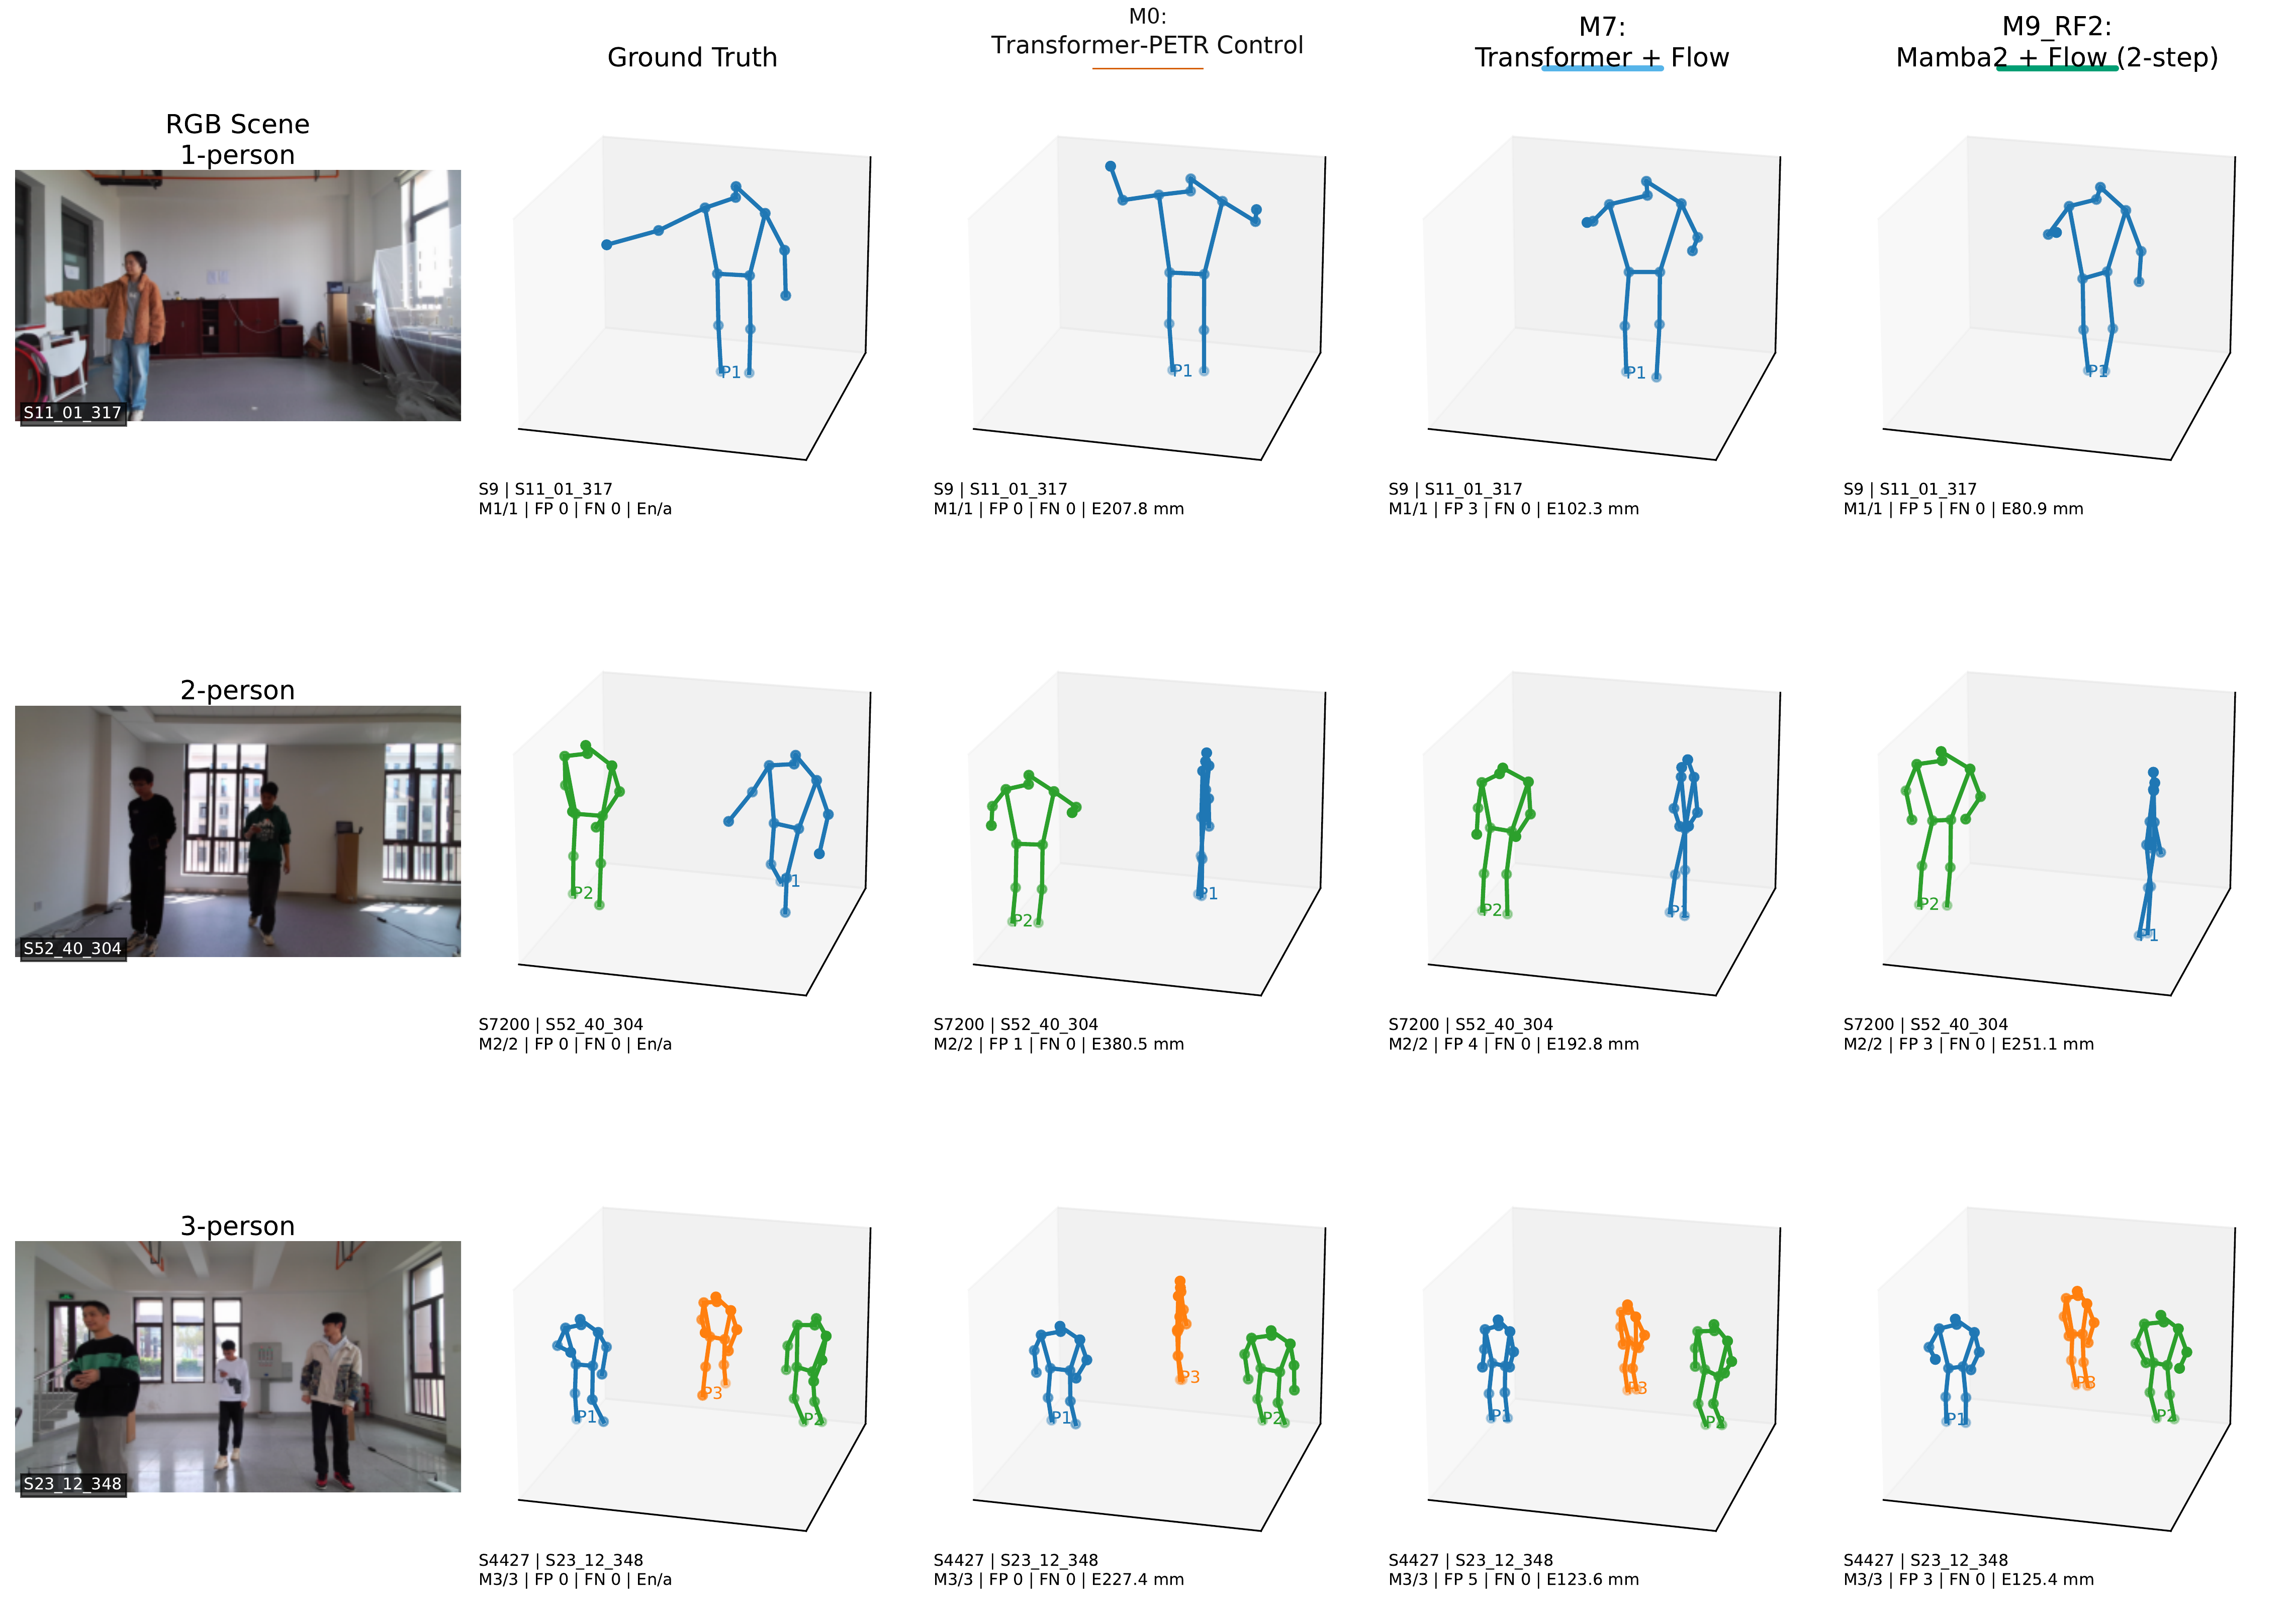
\includegraphics[width=0.99\linewidth]{figures/fig_qualitative_full_paper.png}
        \caption{Selected qualitative WiFi pose samples across 1-person, 2-person, and 3-person settings under the same held-out split as Tables~\ref{tab:main} and~\ref{tab:flow}. Columns show the synchronized RGB scene, Kinect ground truth, Transformer-PETR Control, Transformer Flow, and Mamba-2 Flow (two steps) predictions. Unmatched predictions above the fixed confidence threshold are gray. Panel footers report per-sample matching diagnostics rather than aggregate test metrics.}
    }
    \label{fig:qualitative}
\end{figure}

\section{Discussion}
The controlled contrasts are consolidated in Table~\ref{tab:hypothesis-verdict}. The M0--M1 contrast supports the full Spectral Tokenizer as a representation-level package, but it cannot attribute the observed change specifically to spectral conditioning because normalization and temporal residual processing also change. This is why the mechanism is described as a projected-feature descriptor and learned gate, rather than as a physical Doppler interpretation. The main architectural result is an interaction between sequence modeling and pose-head complexity. Retaining the PETR head prevents the Mamba variants from lowering MPJPE, whereas the flattened Mamba-2 path becomes effective with the lightweight query-pose head. In that compact path, Mamba-2 Draft establishes the throughput--memory endpoint and conditional flow refinement improves localization. This progression is visible across the architecture ladder in Table~\ref{tab:main} and Figure~\ref{fig:main_ablation}.

The flow analysis adds an important distinction to the aggregate MPJPE result. Mamba-2 Draft has fewer unmatched persons and higher throughput, while Mamba-2 Flow (two steps) improves both overall and matched-only MPJPE. The contribution is not flow matching in isolation, but its use as a two-step correction stage for query-conditioned WiFi pose drafts. Under the fixed protocol, the two variants therefore support complementary operating choices rather than competing claims: choose Mamba-2 Draft when throughput and memory dominate, or choose Mamba-2 Flow (two steps) when lowest pose error is the priority (Table~\ref{tab:flow} and Figure~\ref{fig:flow_ablation}).

The supplementary diagnostics bound this interpretation. Figure~\ref{fig:accuracy_efficiency_bubble} places all variants in the accuracy--efficiency space without changing the primary Table~\ref{tab:main} comparison. Table~\ref{tab:per-joint} shows lower MPJPE for 12 of 14 joints for Mamba-2 Flow (two steps), with right wrist and right ankle as the two small exceptions. Table~\ref{tab:receiver-ablation} shows that the intended three-receiver input achieves 165.5 mm MPJPE, while the reported two-receiver masks range from 401.6 to 433.3 mm; this is a sensitivity diagnostic, not a cross-environment generalization claim. Finally, Table~\ref{tab:flow-control} reports separately trained low-flow-loss controls and is not substituted for the same-configuration solver comparison in Table~\ref{tab:flow}.

\begin{table}[!t]
\centering
\caption{Evidence map for the controlled architecture ladder. Effect sizes are derived from Tables~\ref{tab:main} and~\ref{tab:flow}; lower MPJPE and matched MPJPE are better, while higher FPS is better.}
\label{tab:hypothesis-verdict}
\resizebox{\linewidth}{!}{%
\begin{tabular}{l l l l}
\toprule
Claim & Controlled comparison & Effect size & Evidence \\
\midrule
The full Spectral Tokenizer improves the linear control endpoint & Transformer-PETR Control $\rightarrow$ Spectral PETR & $-3.269$ mm MPJPE & Table~\ref{tab:main}, Figure~\ref{fig:main_ablation} \\
Flattened Mamba-2 is effective with the compact head & Transformer Draft $\rightarrow$ Mamba-2 Draft & $-2.223$ mm MPJPE; $+66.9$ FPS & Table~\ref{tab:main}, Figure~\ref{fig:main_ablation} \\
Two Euler steps improve flow localization & Bypassed/one-step $\rightarrow$ two-step flow & $-2.245/-2.599$ mm overall MPJPE & Table~\ref{tab:flow}, Figure~\ref{fig:flow_ablation} \\
Compact drafting plus two-step flow is the accuracy endpoint & Transformer-PETR Control $\rightarrow$ Mamba-2 Flow (2 steps) & $-7.053$ mm MPJPE; $1.77\times$ FPS & Table~\ref{tab:main}, Figure~\ref{fig:main_ablation} \\
\bottomrule
\end{tabular}}
\end{table}

\section{Evaluation Scope}
The controlled ablations use deterministic seed 42 under the shared fixed three-receiver protocol. The reported comparisons therefore characterize architecture trade-offs within this sensing layout and temporal split; they do not make cross-environment or random-initialization variance claims.

\section{Conclusion}
This paper presents a compact draft-to-refine WiFi 3D pose architecture centered on spectrally conditioned temporal residual tokens, flattened Mamba-2 sequence modeling, lightweight query-pose drafting, and two-step conditional flow correction. The tokenizer uses a compact projected-feature spectral descriptor to condition a per-link temporal residual update. Under the shared fixed-layout protocol, Mamba-2 Flow (two steps) achieves the lowest measured MPJPE at 165.487 mm while retaining 209.9 FPS, 3.618M parameters, and 25.29 MB peak allocated memory. Compared with the Transformer-PETR Control, it reduces MPJPE by 7.053 mm while using 72.45\% fewer parameters and 83.75\% less allocated memory. The result supports the subtitle directly: compact drafting plus a small flow correction stage reaches the best observed accuracy--efficiency point without a complex pose-decoding architecture.

\section*{Data and Code Availability}
This work reuses the public benchmark released with \cite{yan2024personwifi3d}. The supplementary material provides the LaTeX source, configuration files, benchmark summaries, and figure scripts for the reported tables and figures.

\section*{Ethics Statement}
The benchmark release used in this study reports ethics clearance for public reuse \cite{yan2024personwifi3d}. We collect no new human-subject data. RGB-D annotations are used only as synchronized pose supervision within the benchmark protocol.

\section*{Author Contributions}
Nguyen Vinh Nghi, Le Ngoc Anh Thu, and Nguyen Ngo Nhat Nam contributed to system design, experiment execution, analysis, and manuscript preparation. Tran Ngoc Hoang supervised the research direction, reviewed the experimental interpretation, and advised the manuscript preparation.

\section*{AI Disclosure}
This manuscript was prepared with the assistance of AI-powered academic writing tools, in compliance with the ResFes 2026 commitment on responsible use of AI. AI assistance covered structure planning, result summarization, figure and table integration, and LaTeX formatting. All claims, numerical results, and conclusions were directed and reviewed by the authors, who take full responsibility for the accuracy and integrity of the work. No part of the experimental data, trained models, or reported metrics was generated by an AI system.

\section*{Acknowledgment}
This work builds on the open benchmark and code released by Yan et al. \cite{yan2024personwifi3d}, together with the RESFES 2026 ablation experiments conducted by the authors.

\appendices
\section{Supplementary Figures}
\label{app:figures}
Figure~\ref{fig:accuracy_efficiency_bubble} reuses the full ablation log from Table~\ref{tab:main} to show the accuracy--efficiency trade-off. It is complementary to the exact numerical comparison in Table~\ref{tab:main}: bubble area denotes parameter count rather than an additional outcome.

\begin{figure}[!ht]
    \centering
    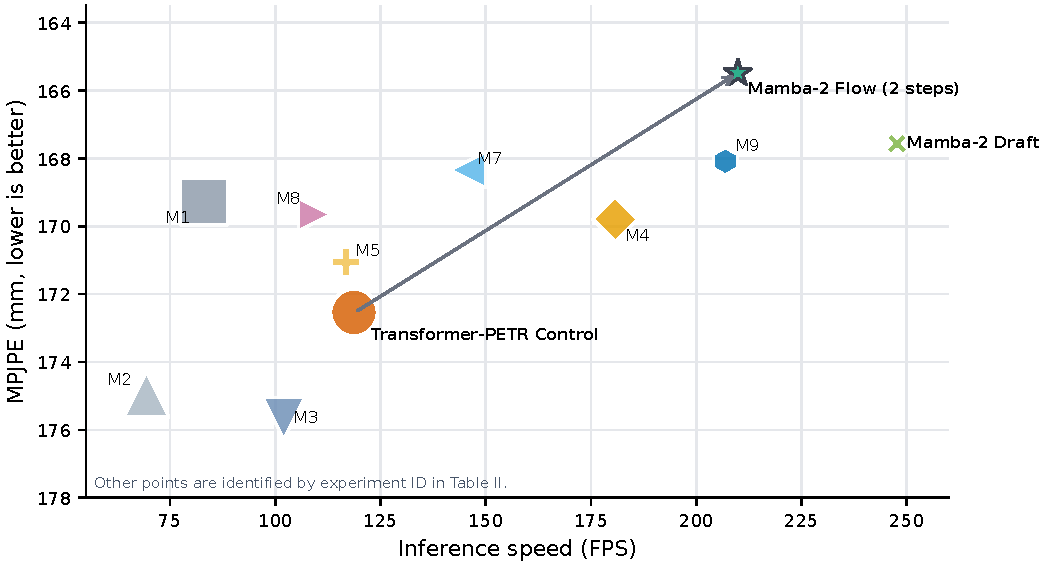
\includegraphics[width=0.88\linewidth]{figures/fig_accuracy_efficiency_bubble.pdf}
\caption{Accuracy--efficiency trade-off of the evaluated variants under the shared fixed-layout protocol. The three functional anchor labels identify the Transformer-PETR Control, the Mamba-2 Draft throughput endpoint, and the Mamba-2 Flow (two steps) accuracy-oriented setting; other points use stable experiment IDs defined in Table~\ref{tab:variant-summary}. Lower MPJPE in millimeters is better, higher model-only FPS is better, and bubble area corresponds to parameter count in millions.}
    \label{fig:accuracy_efficiency_bubble}
\end{figure}

\FloatBarrier
\section{Per-Joint and Receiver Diagnostics}
\label{app:perjoint}
Table~\ref{tab:per-joint} compares Mamba-2 Flow (two steps) with the Transformer-PETR Control at the joint level. The selected model improves 12 of 14 joints; the largest reductions occur at the left hip (10.7 mm), left knee (13.2 mm), and left elbow (12.4 mm), whereas the right wrist increases by 8.4 mm and the right ankle by 0.3 mm. These joint-level values complement, rather than replace, the overall metric in Table~\ref{tab:main}.

\begin{table}[!ht]
\caption{Per-joint MPJPE for Mamba-2 Flow (two steps) versus PETR Reference,
evaluated on the same held-out evaluation set as
Table~\ref{tab:main}. Lower is better. Units: millimeters.}
\label{tab:per-joint}
\centering
\begin{tabular}{l c c}
\toprule
joint & Mamba-2 Flow (2 steps) & PETR Reference \\
\midrule
    neck & 159.2 & 163.0 \\
    head & 147.3 & 154.2 \\
    left shoulder & 155.8 & 162.3 \\
    right shoulder & 155.2 & 161.8 \\
    left elbow & 126.9 & 139.3 \\
    right elbow & 193.5 & 194.0 \\
    left wrist & 128.7 & 138.1 \\
    right wrist & 260.1 & 251.7 \\
    left hip & 128.0 & 146.7 \\
    right hip & 199.9 & 203.2 \\
    left knee & 126.4 & 139.6 \\
    right knee & 124.7 & 142.2 \\
    left ankle & 132.9 & 141.6 \\
    right ankle & 278.3 & 278.0 \\
    \midrule
    \textbf{Mean} & \textbf{165.5} & \textbf{172.6} \\
\bottomrule
\end{tabular}
\end{table}


\FloatBarrier
\section{Receiver-Subset Diagnostic}
\label{app:receiver}
Table~\ref{tab:receiver-ablation} reports the selected model under receiver masking. The full three-receiver input remains the intended fixed-layout operating condition at 165.5 mm MPJPE; the two-receiver subsets range from 401.6 to 433.3 mm, and the R2-only subset reaches 498.0 mm. Subset rows are therefore a compact sensitivity diagnostic, not evidence of cross-environment or cross-subject generalization.

\begin{table}[htbp]
\caption{Per-receiver evaluation of M9\_RF2 on the same test split as
Table~\ref{tab:main}. Receivers not in the subset are zero-masked
at the input of the WiTiDAR pipeline (the model is not retrained).
Mirrors baseline Table~5 of \cite{yan2024personwifi3d}. Units: mm; lower
is better.}
\label{tab:receiver-ablation}
\centering
\begin{tabular}{l c c c c c c}
\toprule
receiver subset & MPJPE & 1P & 2P & 3P & matched & missed \\
\midrule
    3 receivers (R1{+}R2{+}R3) & 165.5 & 121.8 & 159.3 & 190.2 & 15044 & 72 \\
    R1{+}R2 & 401.6 & 382.6 & 407.1 & 403.9 & 9567 & 5549 \\
    R1{+}R3 & 414.1 & 431.2 & 414.7 & 406.2 & 8838 & 6278 \\
    R2{+}R3 & 433.3 & 417.2 & 433.4 & 440.0 & 7828 & 7288 \\
    R2 only & 498.0 & 496.3 & 499.6 & 497.0 & 498 & 14618 \\
\bottomrule
\end{tabular}
\end{table}


\FloatBarrier
\section{Flow-Loss Sensitivity}
\label{app:flow-control}
Table~\ref{tab:flow-control} reports the two low-flow-loss control runs. Their two-step and four-step outcomes are 167.981 and 169.454 mm MPJPE, respectively; these controls are supplementary to, and should not replace, the same-configuration solver analysis in Table~\ref{tab:flow}.

\begin{table}[!ht]
\centering
\caption{Low-flow-loss control runs. Lower overall MPJPE and Matched MPJPE are better; values are in millimeters and use the same 500 mm unmatched-person penalty as Table~\ref{tab:flow}.}
\label{tab:flow-control}
\begin{tabular}{l c c c c c c}
\toprule
Inference & MPJPE & Matched & Missed & 1P & 2P & 3P \\
\midrule
Two steps & 167.981 & 166.082 & 86 & 121.335 & 160.970 & 194.804 \\
Four steps & 169.454 & 167.275 & 99 & 120.505 & 161.851 & 197.854 \\
\bottomrule
\end{tabular}
\end{table}

\FloatBarrier
\bibliographystyle{IEEEtran}
\bibliography{references}

\end{document}
